

\chapter{QUESO Examples}

This chapter assumes that the user has successfully installed QUESO and its dependencies.
%
It presents a variety of  examples of how to use QUESO in order to develop applications that solves a statistical inverse problem,
a statistical forward problem or a combination of both.



The codes listed in this section are quite self-explanatory and print messages
during execution to make clearer which problem they are solving and how. 



\todo{A complete example of an application that uses QUESO to solve a combination of a
SIP and a SFP is in presented in Chapter \ref{ch-appl-example}. The chapter
presents the mathematical models for both the SIP and SFP, the application code,
the options input file and the Makefile to link the code  with QUESO library.}





\section{\texttt{simpleStatisticalInverseProblem}}\label{sec:exemple_sip}

According to the Bayesian paradigm, the unobservable parameters
in a statistical model are treated as random. When no data is available,
a prior distribution is used to quantify our knowledge about the parameter.
When data are available, we can update our prior knowledge using the conditional distribution of parameters, given the data. 
The transition from the prior to the posterior is possible via the Bayes theorem:
\begin{equation*}
\pi_{\text{posterior}}(\boldsymbol{\theta}|\mathbf{d})=\frac{\pi_{\text{prior}}(\boldsymbol{\theta})\pi_{\text{likelihood}}(\mathbf{d}|\boldsymbol{\theta})}{\pi(\mathbf{d})}
\end{equation*}


In this example, suppose a random variable of interest with two parameters $\bv{\theta} \in \mathbb{R}^2$ has a uniform prior distribution, and suppose that a suitable likelihood has normal distribution with mean $\bv{\mu}$ and covariance matrix $\bf{C}$, given by:
\begin{equation}\label{eq-example-mu}
\boldsymbol{\mu} = 
\left(\begin{array}{c}
-1 \\
2
\end{array}\right)
\quad
\text{and}
\quad
\mathbf{C} = 
\left[\begin{array}{cc}
4 & 0 \\
0 & 1
\end{array}\right].
\end{equation}

Therefore, we have: 
\begin{equation*}
\pi_{\text{prior}}(\boldsymbol{\theta}) \varpropto 1
\end{equation*}
and
\begin{equation*}
\pi_{\text{like}}(\boldsymbol{\theta}) \varpropto \exp \left(-\frac{1}{2}\left[(\boldsymbol{\theta}-\boldsymbol{\mu})^T[\mathbf{C}^{-1}](\boldsymbol{\theta}-\boldsymbol{\mu})\right] \right),
\end{equation*}
where
\begin{equation*}
\boldsymbol{\theta} = 
\left(
\begin{array}{c}
\theta_1 \\
\theta_2
\end{array}
\right)\in \mathbb{R}^2.
\end{equation*}
%

Therefore,  posterior PDF is given by:
\begin{equation}\label{eq-example-post}
\pi_{\text{post}}(\boldsymbol{\theta}) \varpropto e^{-\frac{1}{2}\left\{(\boldsymbol{\theta}-\boldsymbol{\mu})^T[\mathbf{C}^{-1}](\boldsymbol{\theta}-\boldsymbol{\mu})\right\}}.
\end{equation}


In this example, we can replace the values for the mean and covariance matrix given in Equation (\ref{eq-example-mu}) into Equation (\ref{eq-example-post}), 
in order to analytically compute both the posterior PDF:
\begin{eqnarray*}\label{eq-example-exact-post}
\pi_{\text{post}}(\boldsymbol{\theta}) & = & \frac{1}{4\pi} \exp\left(-\frac{1}{2}(\boldsymbol{\theta}-\boldsymbol{\mu})^T[\mathbf{C}^{-1}](\boldsymbol{\theta}-\boldsymbol{\mu})\right) \\
                                       & = & \frac{1}{4\pi} \exp\left( -\frac{1}{8}(\theta_1+1)^2 - \frac{1}{2}(\theta_2-2)^2\right), \label{eq-example-exact-joint}
\end{eqnarray*}
and the marginal results for $\theta_1$ and $\theta_2$:
\begin{equation}\label{eq-example-exact-marginal}
\begin{split}
\pi_{\text{post}}(\theta_1) & =  \frac{1}{2\sqrt{2\pi}} \exp\left(-\frac{1}{8}(\theta_1+1)^2 \right), \\
\pi_{\text{post}}(\theta_1) & =  \frac{1}{ \sqrt{2\pi}} \exp\left(-\frac{1}{2}(\theta_2-2)^2 \right). 
\end{split}
\end{equation}



Recall that the posterior PDF given in 
Equation (\ref{eq-example-post}) can be sampled through the expression:
\begin{equation}\label{eq-example-exact-normal}
\boldsymbol{\mu}+\mathbf{C}^{1/2}\mathcal{N}(0,I),
\end{equation}
where $\mathcal{N}(0,I)$ designates a Gaussian joint PDF of zero mean and unit covariance matrix, and
$\mathbf{C}^{1/2}$ is given by:
\begin{equation*}
\mathbf{C}^{1/2} = 
\left[\begin{array}{cc}
2 & 0 \\
0 & 1
\end{array}\right].
\end{equation*}

Thus, in this simple statistical inverse problem, we use QUESO implementation of the Markov chain 
algorithm to sample the posterior \eqref{eq-example-post} via Expression (\ref{eq-example-exact-normal}) and compare the calculated marginal results for $\theta_1$ and $\theta_2$ 
against the analytical formulas given in Equation~(\ref{eq-example-exact-marginal}). 


\paragraph*{Note:} Due to the possilility to compare QUESO sampling algorithms to analytical expressions, this example is also used in the verification procedures and regression tests within QUESO, and it is reproduced in the directory \verb+tests/t02_sip_sfp+.




\subsubsection{Running the example}\label{sec:example_sip}
 

\todo{UPDATE-me} To run the executable provided, enter the following commands:
\begin{lstlisting}[label={},caption={}]
$ cd $HOME/LIBRARIES/QUESO-0.46.0/
$ cd examples/simpleStatisticalInverseProblem
$ rm outputData/*
$ ./exStatisticalInverseProblem_gsl sip.inp    
$ matlab
   $ sip_plot	           # inside matlab
   # press the left button of the mouse at each picture displayed 
   # by 'sip_plot.m', in order to display the next picture
   $ exit	               # inside matlab
$ ls -l outputData/*.png
>>  parameters_samples_plane.png  parameters_PDF.png
\end{lstlisting}

As a result, the user should have created a couple of PNG plots for both
marginal posterior PDFs of all four parameters and samples of first two
parameters on the plane.

\todo{Details ....}

\subsection{Application Code}\label{sec:sip-code}

The program example given in this paper is compatible with version 0.46.0 of QUESO.
The source code for the example is composed of 5 files:
\texttt{example\_main.C} (Listing \ref{code:sip-main-c}),
\texttt{example\_likelihood.h} and \texttt{example\_likelihood.C} (Listings \ref{fig-like-h} and \ref{fig-like-c}),
\texttt{example\_compute.h} and \texttt{example\_compute.C} (Listings \ref{code:sip-compute-h} and \ref{code:sip-compute-c}).


\lstinputlisting[caption=File \texttt{example\_main.C.}, label={code:sip-main-c}, linerange={29-1000}]{../../trunk/examples/simpleStatisticalInverseProblem/src/example_main.C}

\lstinputlisting[caption=File \texttt{example\_likelihood.h}., label={fig-like-h}, linerange={28-1000}]{../../trunk/examples/simpleStatisticalInverseProblem/src/example_likelihood.h}

\lstinputlisting[caption=File \texttt{example\_likelihood.C}., label={fig-like-c}, linerange={29-1000}]{../../trunk/examples/simpleStatisticalInverseProblem/src/example_likelihood.C}

\lstinputlisting[caption=File \texttt{example\_compute.h.}, label={code:sip-compute-h}, linerange={28-1000}]{../../trunk/examples/simpleStatisticalInverseProblem/src/example_compute.h}

\lstinputlisting[caption={File \texttt{example\_compute.C}.}, label={code:sip-compute-c}, linerange={29-1000},numbers=left]{../../trunk/examples/simpleStatisticalInverseProblem/src/example_compute.C}
 


\subsection{Input File}\label{sec:sip-input-file}


QUESO reads an input file for solving statistical problems. In the case of a SIP, it expects a list of options for MCMC,
together with options for QUESO enviroment; such as the amount of processors to be used and the seed for its random algorithms.

The options used for solving this simple SIP are displayed in Listing \ref{code:sip-input-file}.

\lstinputlisting[caption={Options for QUESO library used in application code (Listings \ref{code:sip-main-c}-\ref{code:sip-compute-c}})., 
label={code:sip-input-file},]{../../trunk/examples/simpleStatisticalInverseProblem/tests/test_2013_08_26/example.inp}



\subsection{Create your own Makefile}\label{sec:sip-makefile}

 
Listing \ref{code:ip_makefile} presents a Makefile, named `\texttt{Makefile\_example\_margarida}', that may be used to compile the code and create the executable \verb+simple_sip_example+. Naturally, it must be adapted to the user's settings, i.e., it has to have the correct paths for the user's libraries that have actually been used to compile and install QUESO.

\lstinputlisting[caption={Makefile for the application code in Listings \ref{code:sip-main-c}-\ref{code:sip-compute-c}},  label={code:ip_makefile},language={bash}]{../../trunk/examples/simpleStatisticalInverseProblem/src/Makefile_example_margarida}

Thus, to compile, build and execute the code, the user just needs to run the following commands in the same directory where the files are:
\begin{lstlisting}
$ export LD_LIBRARY_PATH=$LD_LIBRARY_PATH:\
  $HOME/LIBRARIES/gsl-1.15/lib/:\
  $HOME/LIBRARIES/boost-1.53.0/lib/:\
  $HOME/LIBRARIES/hdf5-1.8.10/lib:\
  $HOME/LIBRARIES/QUESO-0.46.0/lib 
$ make -f Makefie_example_margarida 
$ simple_sip_example example.inp
\end{lstlisting}

The `\verb+export+' instruction above is only necessaty if the user has not saved it in his/her `\verb+.bashrc+' file.


\subsection{Data Post-Processing and Visualization}\label{sec:sip-results}


There are a few Matlab-ready commands that are very helpful tools for post-processing the data generated by QUESO when solving statistical inverse problems. This section discusses the results computed by QUESO with the code of Section \ref{sec:sip-code}, and shows how to use Matlab for the post-processing of such results. 

According to the specifications of the input file in Listing~\ref{code:sip-input-file}, a folder named `\verb+outputData+' containing the following files should be created: \verb+display_sub0.txt, ip_filt_chain_sub0.m,+ \verb+ip_raw_chain_sub0.m, sipOutput_sub0.m, ip_filt_chain.m, ip_raw_chain.m+
% \begin{verbatim}
% display_sub0.txt
% ip_filt_chain_sub0.m
% ip_raw_chain_sub0.m
% sipOutput_sub0.m
% ip_filt_chain.m
% ip_raw_chain.m
% \end{verbatim}


The code bellow shows how to load the data provided by Queso during the solution process of the SIP described, in the form of 
chains of positions.

\begin{lstlisting}[caption={Matlab code for loading the data in both raw and filtered chains of the SIP.},{basicstyle=\footnotesize\ttfamily}]
% inside Matlab
>> clear all
>> cd outputData/
>> ip_raw_chain
>> ip_filt_chain
\end{lstlisting}


\subsubsection{Autocorrelation Plots}

The code presented in Listing \ref{matlab:simple_sip_autocorr} uses Matlab function \verb+autocorr+ to generate Figure \ref{fig:simple_sip_autocorrelation_raw_filt}
which presents the autocorrelation of the parameters $\theta_1$ and $\theta_2$ in both cases: raw and filtered chain. Details
of styling the curves have been ommited.



\begin{lstlisting}[label=matlab:simple_sip_autocorr,caption={Matlab code for the autocorrelation plots depicted in Figure \ref{fig:simple_sip_autocorrelation_raw_filt}.},{basicstyle=\footnotesize\ttfamily}]
% inside Matlab
% theta_1
>> nlags=10;
>> [ACF_raw,lags,bounds] = autocorr(ip_mh_rawChain_unified(:,1),nlags,0);
>> [ACF_filt,lags,bounds] = autocorr(ip_mh_filtChain_unified(:,1),nlags,0);
>> plot(lags,ACF_raw,'--*b',lags,ACF_filt,'sb-','linewidth',3);
>> ylabel('Autocorrelation for \theta_1','fontname','Times','fontsize',20);
>> xlabel('Lag','fontname', 'Times', 'fontsize',20);

% theta_2
>> [ACF_raw,lags,bounds] = autocorr(ip_mh_rawChain_unified(:,2),nlags,0);
>> [ACF_filt,lags,bounds] = autocorr(ip_mh_filtChain_unified(:,2),nlags,0);
>> plot(lags,ACF_raw,'ro--',lags,ACF_filt,'r*-','linewidth',3);
>> ylabel('Autocorrelation for \theta_2','fontname','Times','fontsize',20);
>> xlabel('Lag','fontname', 'Times', 'fontsize',20);
\end{lstlisting}

\begin{figure}[htpb]
\centering
\subfigure[$\theta_1$]{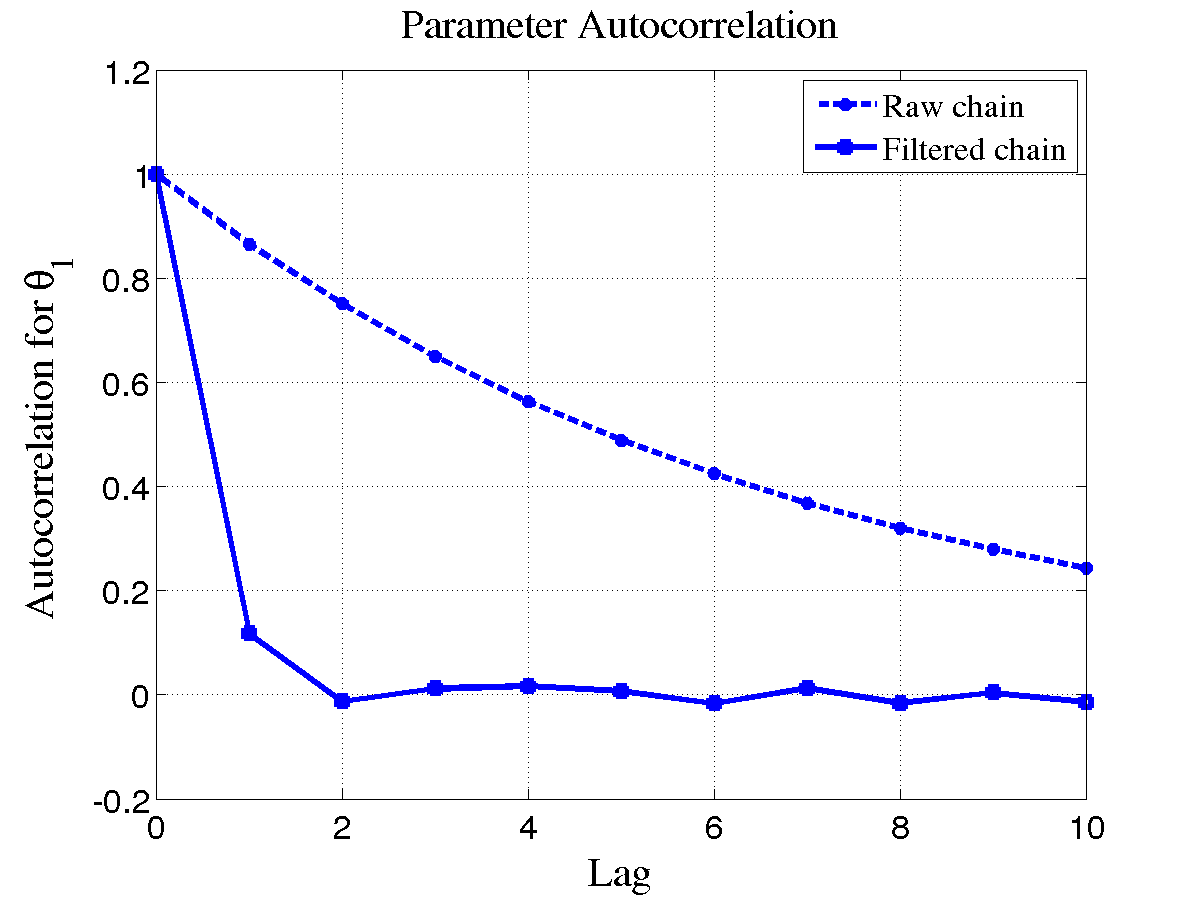
\includegraphics[scale=0.40]{rawfigs/simple_ip_autocorrelation_raw_filt_theta1.png}}
\subfigure[$\theta_2$]{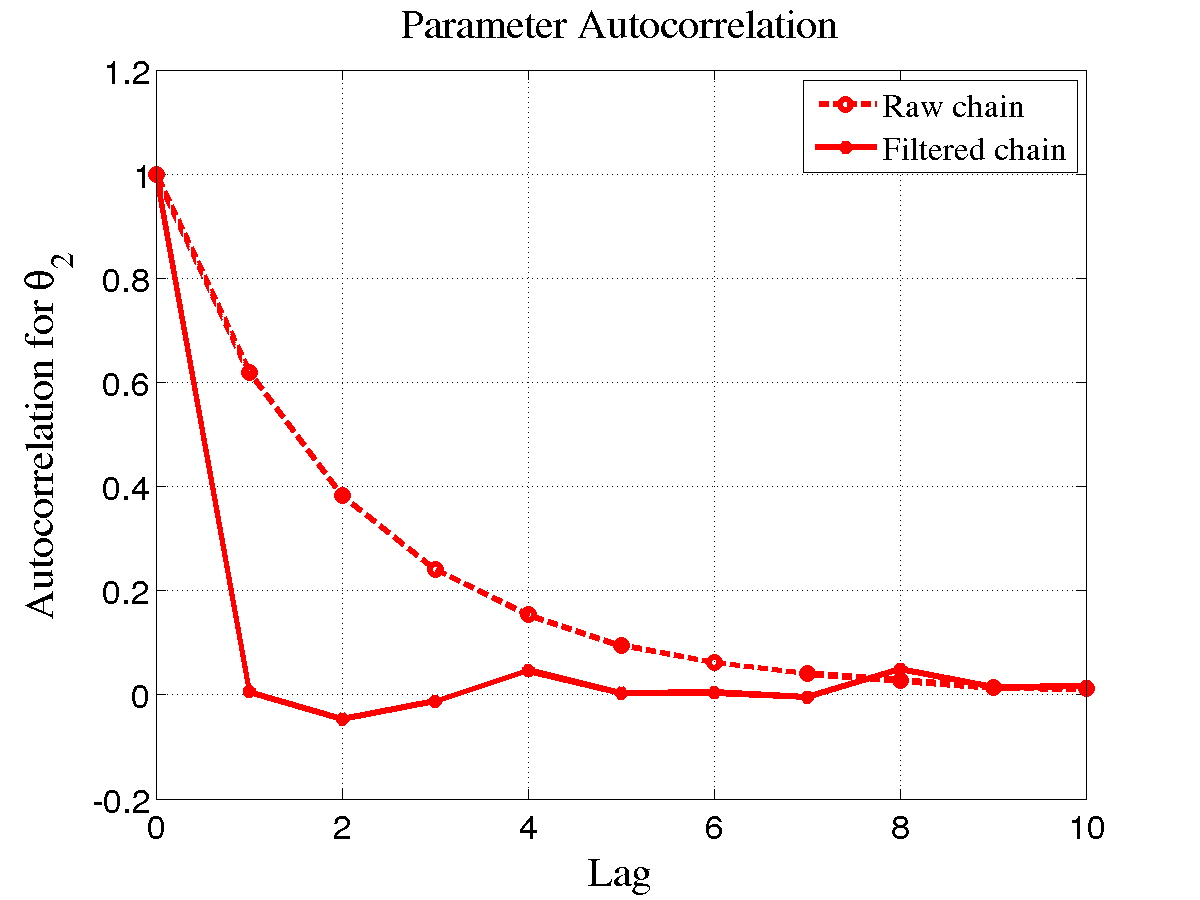
\includegraphics[scale=0.40]{rawfigs/simple_ip_autocorrelation_raw_filt_theta2.png}}
\vspace{-8pt}
\caption{
Autocorrelation plots obtained with QUESO for the SIP. }
\label{fig:simple_sip_autocorrelation_raw_filt}
\end{figure}


\subsubsection{KDE Plots}

Matlab function \verb+[f,xi] = ksdensity(x)+ (kernel smoothing density estimate) computes a probability density estimate of the sample in the vector \texttt{x}. \texttt{f} is the vector of density values evaluated at the points in \texttt{xi}. The estimate is based on a normal kernel function, using a window parameter (`width') that is a function of the number of points in \texttt{x}. The density is evaluated at 100 equally spaced points that cover the range of the data in x.  In order to estimate the KDE of the parameters, it is used together with the option `\verb+pdf+'. 

\begin{lstlisting}[label=matlab:ip_kde,caption={Matlab code for the KDE plots displayed in Figure \ref{fig:simple_sip_kde}.},{basicstyle=\footnotesize\ttfamily}]
% inside Matlab
% theta_1
>> [f,xi] = ksdensity(ip_mh_rawChain_unified(:,1),'function','pdf');
>> x=ip_mh_rawChain_unified(:,1);
>> x=sort(x);
>> plot(x,(exp(-(x+1).*(x+1)/8))/2/sqrt(2*pi),'--k',xi,f,'-b','linewidth',3);
>> title('Parameter Kernel Density Estimation (raw chain)','fontname', 'Times', 'fontsize',20);
>> ylabel('Posterior marginal PDF','fontname', 'Times', 'fontsize',20);
>> xlabel('\theta_1','fontname', 'Times', 'fontsize',20);
>> h=legend('Analytical','QUESO','location','northeast');

% theta_2
>> fprintf(1,' Plotting KDE - raw  <press any key>\n');
>> [f,xi] = ksdensity(ip_mh_rawChain_unified(:,2),'function','pdf');
>> x=ip_mh_rawChain_unified(:,2);
>> x=sort(x);
>> plot(x,(exp(-(x-2).*(x-2)/2))/sqrt(2*pi),'--k',xi,f,'-r','linewidth',3);
>> title('Parameter Kernel Density Estimation (raw chain)','fontname', 'Times', 'fontsize',20);
>> ylabel('Posterior marginal PDF','fontname', 'Times', 'fontsize',20);
>> xlabel('\theta_2','fontname', 'Times', 'fontsize',20);
>> h=legend('Analytical','QUESO','location','northeast');
\end{lstlisting}

%Figure \ref{fig:sip_gravity_kde_raw} is created by using Matlab commands presented in Listing \ref{matlab:kde} above.
\begin{figure}[htpb]
\centering 
\subfigure[]{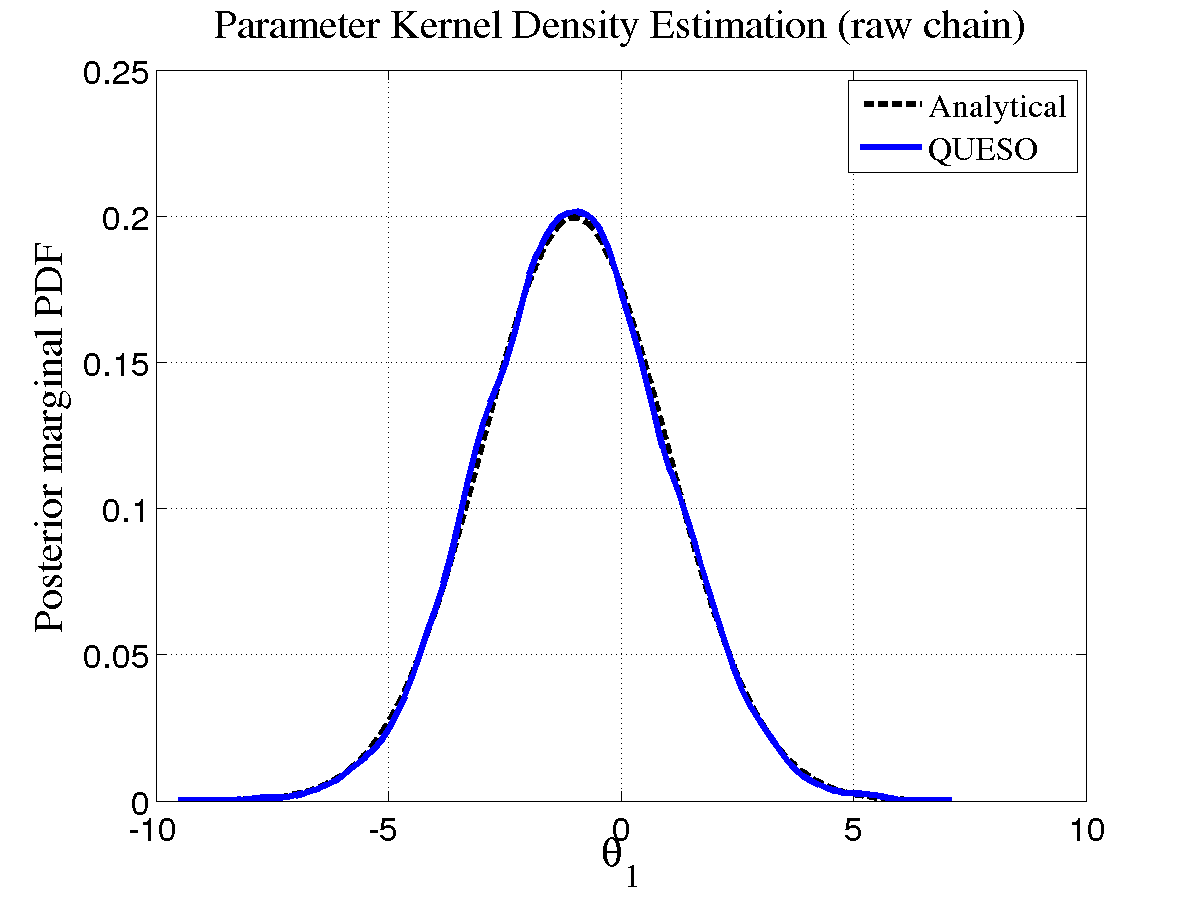
\includegraphics[scale=0.35]{rawfigs/simple_ip_kde_theta1.png}}
\subfigure[]{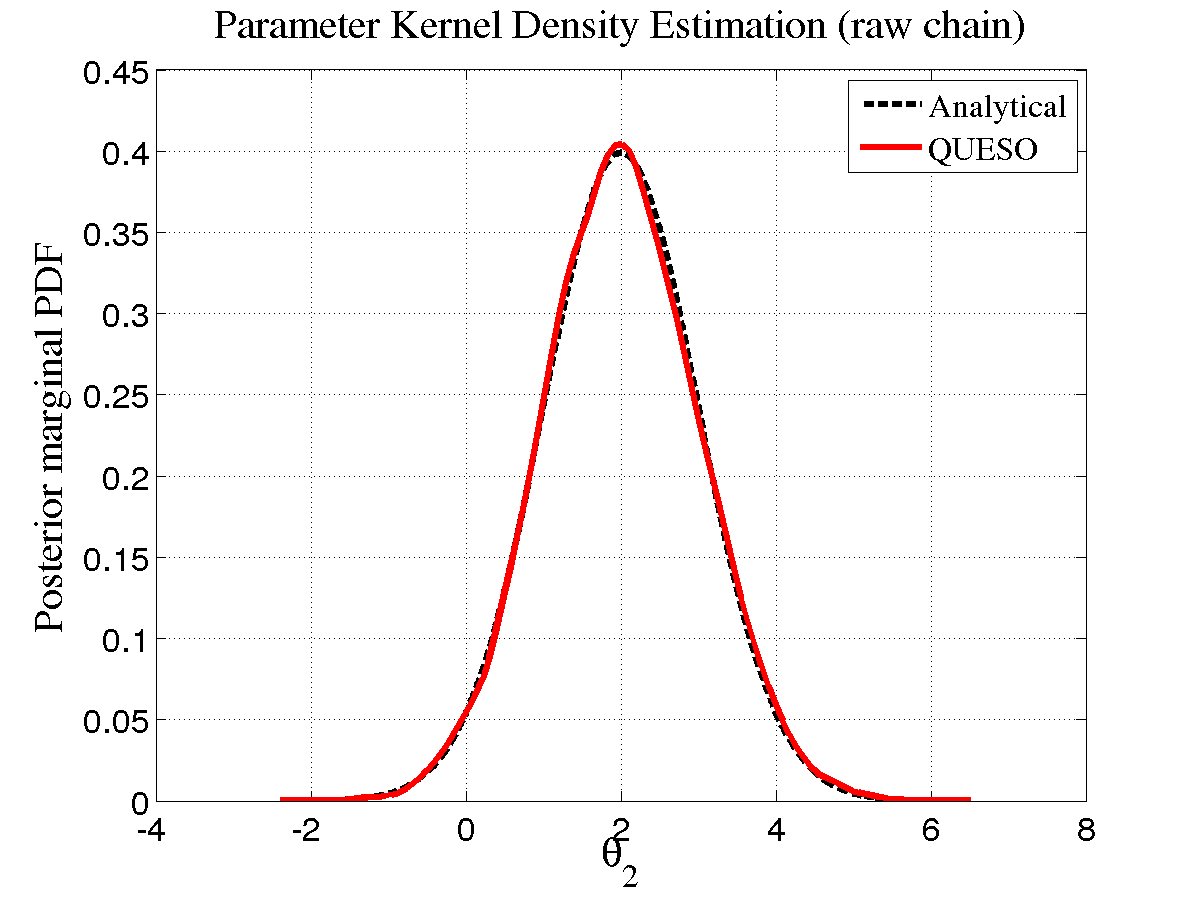
\includegraphics[scale=0.35]{rawfigs/simple_ip_kde_theta2.png}}
\vspace*{-10pt}
\caption{Kernel Density Estimation. In (a), QUESO results are plotted against the analitical expression $\pi_{\text{post}}(\theta_1)  =  \frac{1}{2\sqrt{2\pi}} \exp\left(-\frac{1}{8}(\theta_1+1)^2 \right)$; in (b), QUESO results are plotted against $\pi_{\text{post}}(\theta_1)  =  \frac{1}{ \sqrt{2\pi}} \exp\left(-\frac{1}{2}(\theta_2-2)^2 \right)$.}
\label{fig:simple_sip_kde}
\end{figure}



\subsubsection{Covariance and Correlation Matrices}

Matlab function \verb+cov+ calculates the covariance matrix for a data matrix (where each column represents a separate quantity), 
and \verb+corr+ calculates the correlation matrix.

Listing \ref{matlab:cov_matrix} presents the Matlab steps for calculating the covariance and correlation matrices for the parameterss $\theta_1$ and $\theta_2$.
\begin{lstlisting}[label=matlab:ip_cov_matrix,caption={Matlab code for finding covariance and correlation matrices.},{basicstyle=\footnotesize\ttfamily}]
% inside Matlab
>> cov_matrix_theta1_theta2 = cov(ip_mh_rawChain_unified)

cov_matrix_theta1_theta2 =

    3.8729    0.0259
    0.0259    1.0050
    
>> corr_matrix_theta1_theta2 = corr(ip_mh_rawChain_unified)

corr_matrix_theta1_theta2 =

    1.0000    0.0132
    0.0132    1.0000    
\end{lstlisting}

\section{\texttt{simpleStatisticalForwardProblem}}

In this simple statistical forward problem (SFP), suppose that the quantity of interest $\mathbf{q}$ is a function of a random variable $\bv{\theta}$ of two parameters, namely $\bf{q}:\mathbb{R}^2\rightarrow\mathbb{R}$ such as:
\begin{equation}\label{eq-example-q}
\mathbf{q}(\boldsymbol{\theta}) = \theta_1+\theta_2,\quad\forall\boldsymbol{\theta}=(\theta_1,\theta_2)\in\mathbb{R}^2.
\end{equation}

Suppose also that the parameters in $\theta$ have Gaussian distribution with mean $\bv{\mu}$ and covariance matrix $\bf{C}$ given by:
\begin{equation}\label{eq-example-mu-sfp}
\boldsymbol{\mu} = 
\left(\begin{array}{c}
-1 \\
2
\end{array}\right)
\quad
\text{and}
\quad
\mathbf{C} = 
\left[\begin{array}{cc}
4 & 0 \\
0 & 1
\end{array}\right].
\end{equation}


Notice that since the solution $\mathbf{Q}$ of this SFP is the sum of two random variables $\boldsymbol{\Theta}_1$ and $\boldsymbol{\Theta}_2$, and since these two random variables independent Gaussian by assumption, should have:
\begin{equation}\label{eq-example-E}
E[\mathbf{Q}] = E[\boldsymbol{\Theta}_1] + E[\boldsymbol{\Theta}_2] = -1 + 2 = 1
\end{equation}
and
\begin{equation}\label{eq-example-V}
V[\mathbf{Q}] = V[\boldsymbol{\Theta}_1] + V[\boldsymbol{\Theta}_2] = 4 + 1 = 5
\end{equation}
where $E$ and $V$ indicate expectation and variance, respectively. Thus the analytical expression for the solution $\bf{Q}$ is this SFP is the one-dimensional Gaussian distribution of mean 1 and variance 5:
\begin{equation}\label{eq-example-sfp-analytical}
{\bf Q}(x)=   \frac{1}{ \sqrt{10\pi}} \exp\left(-\frac{1}{10}(x-1)^2 \right)
\end{equation}


In this example, we use QUESO Monte Carlo algorithm to sample from the QoI given in Equation (\ref{eq-example-q}) and analyse it. 
Since the parameters have known independent Guassian distributions, the results obtained by QUESO via sampling the QoI, in Equation (\ref{eq-example-q}), should match the Gaussian distribution given in Equation (\ref{eq-example-sfp-analytical}).


\paragraph*{Note:} Due to the possilility to compare QUESO sampling algorithms to an analytical expression, this example is also used in the verification procedures and regression tests within QUESO. In fact it is the second part of the test \verb+tests/t02_sip_sfp+.


\subsection{Running the example}\label{sec:example_sfp}
 

\todo{UPDATE-me} To run the executable provided, enter the following commands:
\begin{lstlisting}[label={},caption={}]
$ cd $HOME/LIBRARIES/QUESO-0.46.0/
$ cd examples/simpleStatisticalForwardProblem
$ rm outputData/*
$ ./exStatisticalInverseProblem_gsl sip.inp    
$ matlab
   $ sip_plot	           # inside matlab
   # press the left button of the mouse at each picture displayed 
   # by 'sip_plot.m', in order to display the next picture
   $ exit	               # inside matlab
$ ls -l outputData/*.png
>>  parameters_samples_plane.png  parameters_PDF.png
\end{lstlisting}

As a result, the user should have created a couple of PNG plots for both
marginal posterior PDFs of all four parameters and samples of first two
parameters on the plane.

\todo{Details ....}



\subsection{Application Code}\label{sec:code-sfp}


The program example given in this paper is compatible with version 0.46.0 of QUESO.
The source code for the example is composed of 5 files:
\texttt{simple\_sfp\_example\_main.C} (Listing \ref{code:sfp-main-c}),
\texttt{simple\_sfp\_example\_qoi.h} and \texttt{simple\_sfp\_example\_qoi.C} (Listings \ref{code:sfp-qoi-h} and \ref{code:sfp-qoi-c}),
\texttt{simple\_sfp\_example\_compute.h}  and \texttt{simple\_sfp\_example\_compute.C} (Listings \ref{code:sfp-compute-h} and \ref{code:sfp-compute-c}).


\lstinputlisting[caption=File \texttt{example\_main.C.}, label={code:sfp-main-c}, linerange={29-1000}]{../../trunk/examples/simpleStatisticalForwardProblem/src/simple_sfp_example_main.C}

\lstinputlisting[caption=File \texttt{example\_qoi.h}., label={code:sfp-qoi-h}, linerange={28-1000}]{../../trunk/examples/simpleStatisticalForwardProblem/src/simple_sfp_example_qoi.h}

\lstinputlisting[caption=File \texttt{example\_qoi.C}., label={code:sfp-qoi-c}, linerange={29-1000}]{../../trunk/examples/simpleStatisticalForwardProblem/src/simple_sfp_example_qoi.C}

\lstinputlisting[caption=File \texttt{example\_compute.h.}, label={code:sfp-compute-h}, linerange={28-1000}]{../../trunk/examples/simpleStatisticalForwardProblem/src/simple_sfp_example_compute.h}

\lstinputlisting[caption={File \texttt{example\_compute.C}.}, label={code:sfp-compute-c}, linerange={29-1000},numbers=left]{../../trunk/examples/simpleStatisticalForwardProblem/src/simple_sfp_example_compute.C}
 


\subsection{Input File}\label{sec:sfp-input-file}

In the case of a SFP, QUESO expects a list of options for Monte Carlo algorithm,
together with options for QUESO enviroment; such as the name of the output files and which sub-enviroments will write to to them. 
The options used for solving this simple SFP are displayed in Listing \ref{code:sfp-input-file}.


\lstinputlisting[caption={File name \texttt{simple\_sfp\_example.inp} with options for QUESO library used in application code (Listings \ref{code:sip-main-c}-\ref{code:sip-compute-c}})., 
label={code:sfp-input-file},]{../../trunk/examples/simpleStatisticalForwardProblem/tests/test_2013_08_27/simple_sfp_example.inp}



\subsection{Create your own Makefile}\label{sec:sfp-makefile}

 
Listing \ref{code:makefile} presents a Makefile, named `\texttt{Makefile\_sfp\_example\_margarida}', that may be used to compile the code and create the executable \verb+simple_sfp_example+. Naturally, it must be adapted to the user's settings, i.e., it has to have the correct paths for the user's libraries that have actually been used to compile and install QUESO.

\lstinputlisting[caption={Makefile for the application code in Listings \ref{code:sfp-main-c}-\ref{code:sfp-compute-c}},  label={code:sfp-makefile},language={bash}]{../../trunk/examples/simpleStatisticalForwardProblem/src/Makefile_sfp_example_margarida}

Thus, to compile, build and execute the code, the user just needs to run the following commands in the same directory where the files are:
\begin{lstlisting}
$ export LD_LIBRARY_PATH=$LD_LIBRARY_PATH:\
  $HOME/LIBRARIES/gsl-1.15/lib/:\
  $HOME/LIBRARIES/boost-1.53.0/lib/:\
  $HOME/LIBRARIES/hdf5-1.8.10/lib:\
  $HOME/LIBRARIES/QUESO-0.46.0/lib 
$ cd HOME/LIBRARIES/QUESO-0.46.0/examples/simpleStatisticalForwardProblem 
$ make -f Makefile_sfp_example_margarida 
$ cd ../test/test_2013_08_27
$ ../../src/simple_sfp_example simple_sfp_example.inp
\end{lstlisting}

The `\verb+export+' instruction above is only necessaty if the user has not saved it in his/her `\verb+.bashrc+' file.


\subsection{Data Post-Processing and Visualization}\label{sec:sfp-results}


There are a few Matlab-ready commands that are very helpful tools for post-processing the data generated by QUESO when solving SFPs. This section discusses the results computed by QUESO with the code of Section \ref{sec:code-sfp}, and shows how to use Matlab for the post-processing of such results. 

According to the specifications of the input file in Listing~\ref{code:sip-input-file}, a folder named `\verb+outputData+' containing the following files should be created: \verb+display_sub0.txt, fp_p_seq.m,+ \linebreak \verb+fp_p_seq_sub0.m, fp_q_seq.m, fp_q_seq_sub0.m,+ and \verb+sfpOutput_sub0.m+.

The code bellow shows how to load the data provided by Queso during the solution process of the SIP described, in the form of 
chains of positions.

\begin{lstlisting}[caption={Matlab code for loading the data in both parameter and QoI chains of the SFP.},{basicstyle=\footnotesize\ttfamily}]
% inside Matlab
>> clear all
>> cd outputData/
>> fp_p_seq
>> fp_q_seq
\end{lstlisting}



\subsubsection{Histogram Plots}

In order to plot a histogram of the QoI, you may use the pre-defined Matlab function \verb+hist+.
The Matlab code presented in Listing \ref{matlab:fp_hist_qoi} below shows how to create the Figure~\ref{fig:fp_qoi_hist}.

\begin{lstlisting}[label=matlab:fp_hist_qoi,caption={Matlab code for the QoI histogram plot.}]
% inside Matlab
>> fp_q_seq
>> nbins=50;
>> hist(fp_mc_QoiSeq_unified,nbins);
>> title('QoI Histogram','fontsize',20);
>> xlabel('QoI=\theta_1+\theta_2','fontname', 'Times', 'fontsize',20)
>> ylabel('Frequency','fontsize',20);
\end{lstlisting}

\begin{figure}[htb]
\centering 
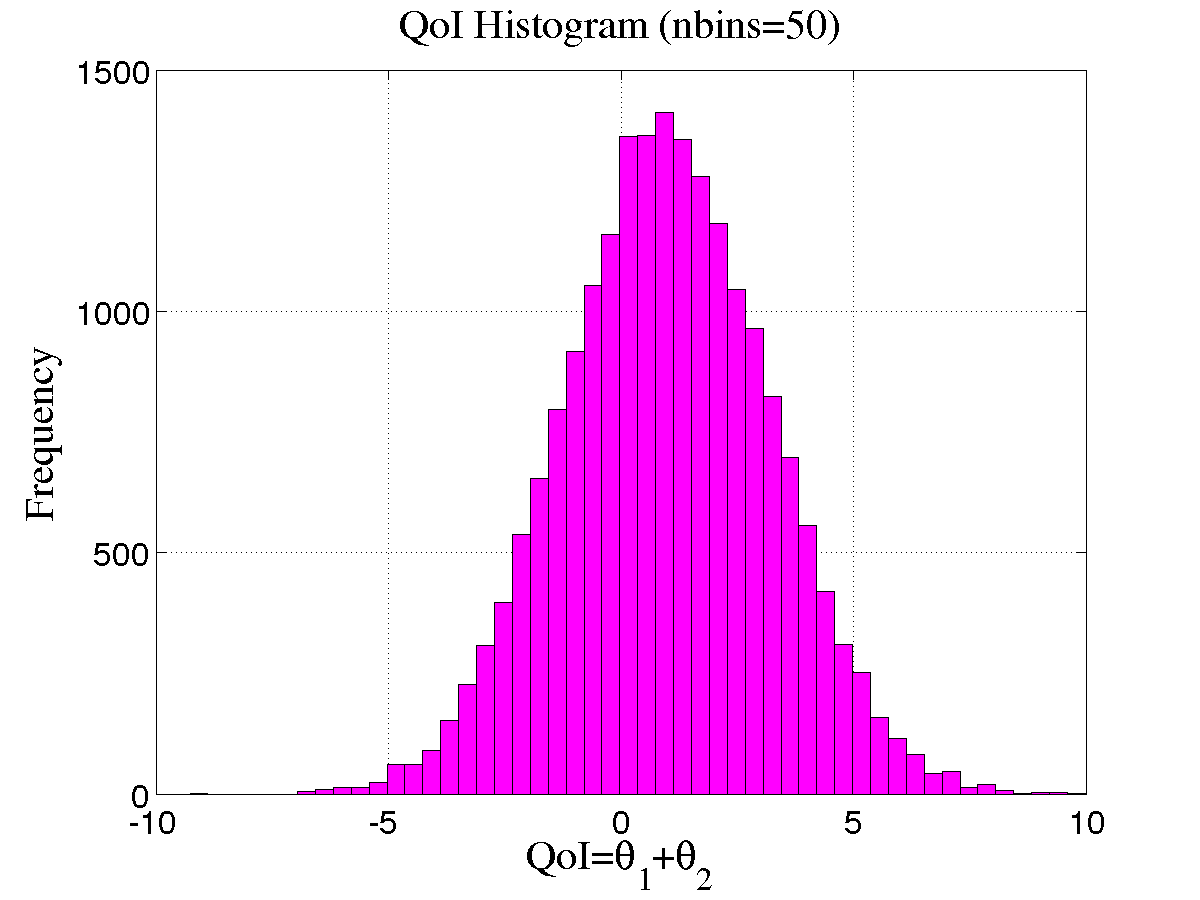
\includegraphics[scale=0.35]{rawfigs/simple_fp_qoi_hist.png}
\vspace{-10pt}
\caption{QoI histogram.}
\label{fig:fp_qoi_hist}
\end{figure}

\subsubsection{KDE Plot}

Matlab function \verb+ksdensity+ (Kernel smoothing density estimate) together with the option `\verb+pdf+' may be used to estimate the KDE of the QoI. 

\begin{lstlisting}[label=matlab:fp_kde_qoi,caption={Matlab code for the KDE displayed in Figure \ref{fig:simple_sfp_kde}},{basicstyle=\footnotesize\ttfamily}]
% inside Matlab
>> fp_q_seq
>> [f,xi] = ksdensity(fp_mc_QoiSeq_unified,'function','pdf');
>> x=fp_mc_QoiSeq_unified;
>> mu=1;
>> sigma2=5;
>> plot(x,(exp(-(x-mu).*(x-mu)/sigma2/2))/sqrt(2*pi*sigma2),'--k',xi,f,'-m','linewidth',3);
>> title('QoI Kernel Density Estimation','fontname','Times','fontsize',20);
>> xlabel('QoI = \theta_1 + \theta_2','fontname', 'Times', 'fontsize',20);
>> ylabel('PDF','fontname', 'Times', 'fontsize',20);
>> h=legend('Analytical','QUESO','location','northeast');
\end{lstlisting}


%Figure \ref{fig:sip_gravity_kde_raw} is created by using Matlab commands presented in Listing \ref{matlab:kde} above.
\begin{figure}[htpb]
\centering 
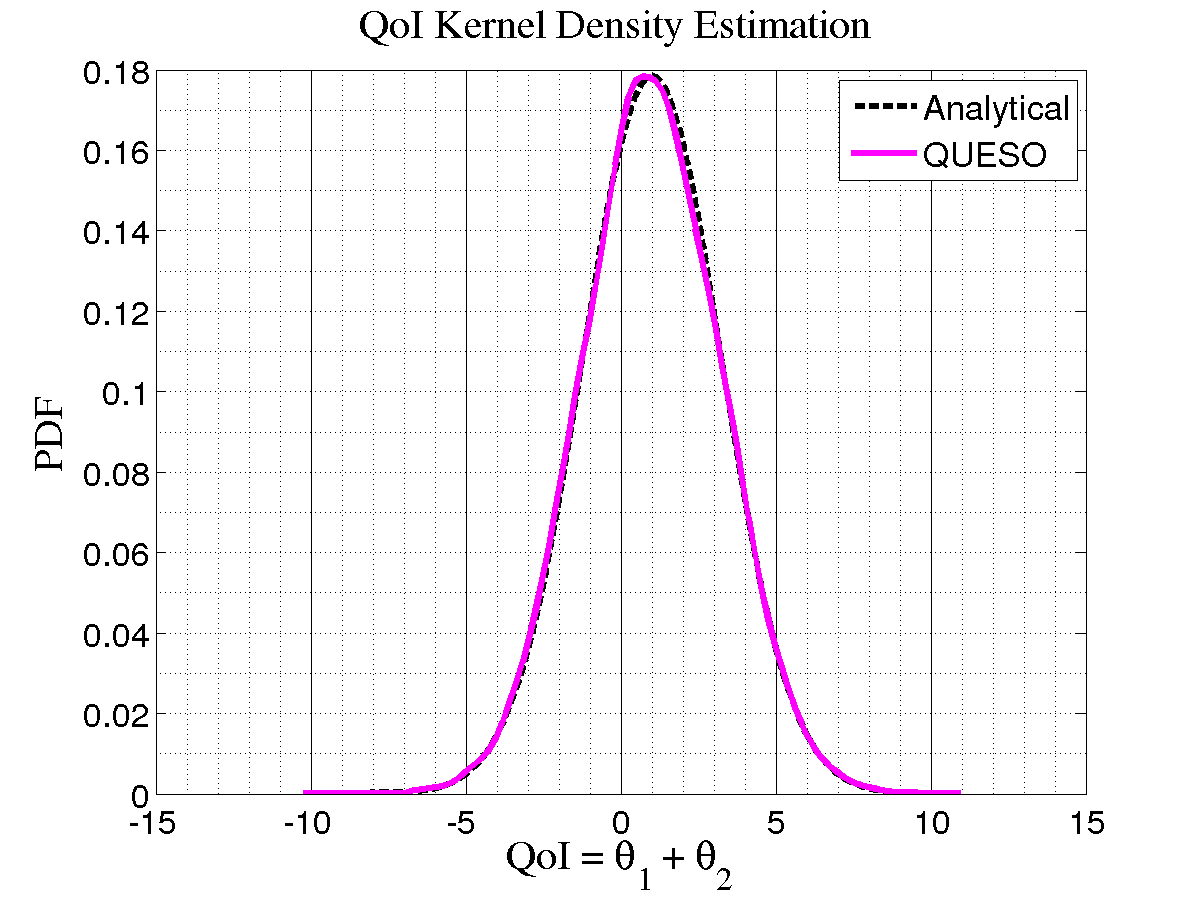
\includegraphics[scale=0.35]{rawfigs/simple_fp_qoi_kde.png}
\vspace{-10pt}
\caption{Kernel Density Estimation. QUESO results are plotted against the PDF of a Gaussian distribution $Q(x)=   \frac{1}{ \sqrt{10\pi}} \exp\left(-\frac{1}{10}(x-1)^2 \right)$, where $\mu=1$ and $\sigma^2=5$.}
\label{fig:simple_sfp_kde}
\end{figure}


\subsubsection{CDF Plot}

Matlab function \verb+ksdensity+ with \verb+'cdf'+ option may also be used for plotting the Cumulative Distribution Function of the QoI.

\begin{lstlisting}[label=matlab:fp_cdf_qoi,caption={Matlab code for the QoI CDF plot displayed in Figure \ref{fig:simple_sfp_cdf}.},{basicstyle=\footnotesize\ttfamily}]
% inside Matlab
>> fp_q_seq
>> [f,xi] = ksdensity(fp_mc_QoiSeq_unified,'function','cdf');
>> plot(xi,f,'-b','linewidth',3)
>> title('QoI Cumulative Distribution Function ','fontsize',20);
>> xlabel('QoI = \theta_1 + \theta_2','fontname', 'Times', 'fontsize',20);
>> ylabel('PDF','fontname', 'Times', 'fontsize',20);
\end{lstlisting}

\begin{figure}[htb]
\centering 
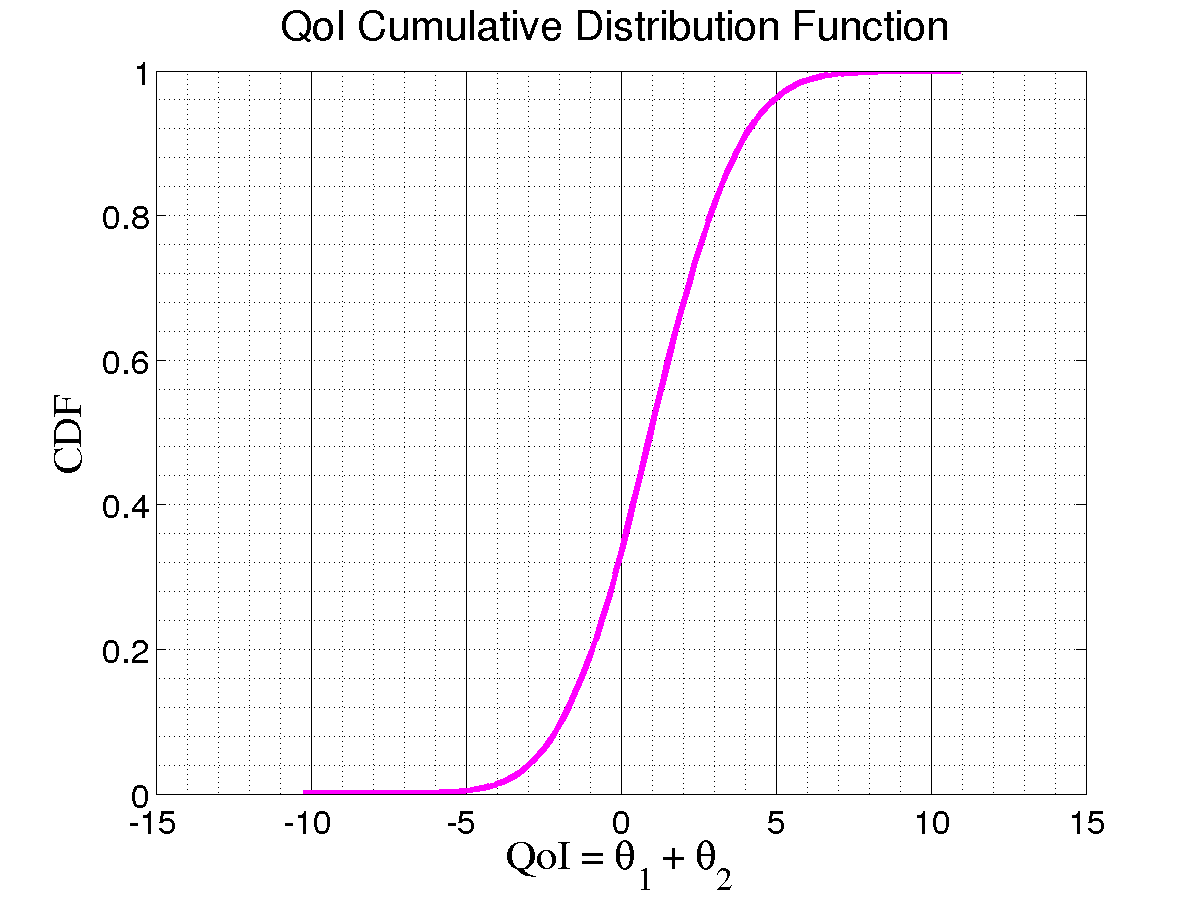
\includegraphics[scale=0.35]{rawfigs/simple_fp_qoi_cdf.png}
\vspace*{-10pt}
\caption{Cumulative Distribution Function.}
\label{fig:simple_sfp_cdf}
\end{figure}

%%%%%%%%%%%%%%%%%%%%%%%%%%%%%%%%%%%%%%%%%%%%%%%%%%%%%%

\chapter{An Application Example}\label{ch-appl-example}
\thispagestyle{headings}
\markboth{Chapter \ref{ch-appl-example}: An Application Example}{Chapter \ref{ch-appl-example}: An Application Example}

This chapter presents an example of how to use QUESO in order to develop an application that solves a statistical inverse problem and
a statistical forward problem, where the solution of the former serves as input to the later.


Section \ref{sec:sip} gives the mathematical formulation of the statistical inverse problem, and presents the required tools and approach for solving it (experimental data, Bayesian approach, and a short overview of DRAM algorithm). Section \ref{sec:sfp} gives the mathematical formulation of the statistical forward problem, its input RV and QoI function, and indicates the statistical method for its solution, the Monte Carlo algorithm.


Section \ref{sec:application_code} presents the codes that translate the mathematical language into C++ using the QUESO classes and algorithms; Section \ref{sec:application_input_file} shows the input file that contains  a list of options for the Markov chain algorithm  (SIP) and the Monte Carlo
algorithm (SFP) which will be used by QUESO classes and algorithms. Instructions on how to compile and run the code are presented in Section \ref{sec:application_compilation}.  Finally, Section \ref{sec:application_results} shows how to plot figures using Matlab and the output data generated by the application.
All the program examples provided in this document are compatible with QUESO \QUESOversion{}. 

%\clearpage
\section{A Statistical Inverse Problem}\label{sec:sip}
% 
% The example described in this section consist of a statistical inverse problem and a statistical forward problem. The statistical inverse problem infers the  acceleration due to gravity for an object in free fall near the surface of the Earth. The statistical forward problem uses such inferred acceleration of gravity to propagate uncertainty in the calculation the motion of an object in projectile movement.


The example described in this section consists of a statistical inverse problem which infers the  acceleration due to gravity for an object in free fall near the surface of the Earth. Later, the inferred acceleration of gravity will be used in a statistical forward problem to propagate uncertainty in the calculation the motion of an object in projectile movement.


\subsection{Mathematical Model for the Statistical Inverse Problem}

% Near the surface of the Earth, an object in free fall in a vacuum will accelerate at approximately $9.8 m/s^2$, independent of its mass.
% With air resistance acting upon an object that has been dropped, mass, drag coefficient and even relative surface may become important
% (if the fall is from sufficient altitude) in the calculation of gravity.

%The vertical motion of an object falling a small distance close to the surface of the planet can be approximated to have
%uniform gravitational field without air resistance, as long as the force of gravity on the object is much greater than the force of air resistance.

%Therefore a convenient, simplified 
A possible deterministic mathematical model for the vertical motion of an object in free fall near the surface of the Earth is given by
\begin{equation}\label{eq:gravity01}
h(t)=-\frac{1}{2} g t^2 + v_0 t + h_0.
\end{equation}
where
$v_0$ [$m/s$] is the initial velocity,
$h_0$ [$m$] is the initial altitude,
$h(t)$ [$m$] is the altitude with respect to time,
$t$ [$s$] is the elapsed time, and
$g$ [$m/s^2$] is the magnitude of the acceleration due to gravity (the parameter which cannot be directly measured and will be statistically inferred).



\subsection{Experimental Data}
We assume that the experiment of allowing an object to fall from different altitudes with zero initial velocity has been repeatedly conducted (See Figure \ref{fig:free_fall}). The data collected, e.g.  $\mathbf{d}$, is displayed in Table \ref{table:data}; the standard deviations, $\sigma$'s, refer to the uncertainties in the measured times during the experiment execution~\cite{interactagram}. 



\begin{figure}[!h]
\centering
\input{rawfigs/free_fall.latex}
\vspace*{-8pt}
\caption{An object falls from altitude $h_0$ with zero initial velocity ($v_0=0$).}
\label{fig:free_fall}
\end{figure}

\begin{table}[htp]%% Data from data02.dat 
\caption{Measurement data $\mathbf{d}$ of size $n_d=14$.
The object falls from altitude $h_0$ in $t$ seconds, with standard deviation of $\sigma$ seconds in the time measurement~\cite{interactagram}.
}
% \specialrule{.4pt}{10pt}{4pt}
\vspace{-8pt}
\begin{center}
\begin{tabular}{ccc}
\toprule
% $(h_0-h)$ [$m$] & $t$ [$s$]  & $\sigma$ [$s$]\\
altitude [$m$] & time [$s$]  & Std. Dev. $\sigma$ [$s$]\\
\midrule
\midrule
$~$10	&	1.41	&	0.02	\\
$~$20	&	2.14	&	0.12	\\
$~$30	&	2.49	&	0.02	\\
$~$40	&	2.87	&	0.01	\\
$~$50	&	3.22	&	0.03	\\
$~$60	&	3.49	&	0.01	\\
$~$70	&	3.81	&	0.03	\\
$~$80	&	4.07	&	0.03	\\
$~$90	&	4.32	&	0.03	\\
100	&	4.47	&	0.05	\\
110	&	4.75	&	0.01	\\
120	&	4.99	&	0.04	\\
130	&	5.16	&	0.01	\\
140	&	5.26	&	0.09	\\
\bottomrule
\end{tabular}
\end{center}
\label{table:data}
\end{table}



\subsection{The Prior RV, Likelihood and Posterior RV}

In a straightforward classical interpretation of Bayesian inference, the prior signifies the modeler's honest opinion about the unknown.
For the gravity inference problem, let's assume that gravity varies uniformly in the interval [8,11], or, in other words, we chose uniform prior distribution in that interval:

\begin{equation}\label{eq-g-prior}
\pi_{\text{prior}}=\mathcal{U}(8,11).
\end{equation}


We choose the usual likelihood function:
\begin{equation}\label{eq:like02}
\pi_{\text{like}}(\mathbf{d} | \boldsymbol{\theta})
\varpropto
\exp
\left\{
-\frac{1}{2}
[\mathbf{y}(\boldsymbol{\theta})-\mathbf{d}]^T
\left[\mathbf{C}(\boldsymbol{\theta})\right]^{-1}
[\mathbf{y}(\boldsymbol{\theta})-\mathbf{d}]
\right\},
\end{equation}
where $\mathbf{C}(\boldsymbol{\theta})$ is a given covariance matrix, $\mathbf{d}$ denotes experimental data, $\mathbf{y}(\boldsymbol{\theta})$ is the model output data.

Recalling the deterministic model for the acceleration of gravity (\ref{eq:gravity01}) with zero initial velocity,  the information provided in Table \ref{table:data}, and Equation (\ref{eq:like02}); and, additionally, invoking the nomenclature used in Section \ref{sec:statistical_concepts}, we have:
\begin{equation}\label{eq:like03}
\boldsymbol{\theta} \stackrel{\text{\small{def.}}}{=} g,
%------------ 
\quad
\mathbf{y}(\boldsymbol{\theta})= 
\left[
\begin{array}{c}
\sqrt{\dfrac{2 h_1}{g}}\\	
\sqrt{\dfrac{2 h_2}{g}}\\	
\vdots\\	
\sqrt{\dfrac{2 h_{n_d}}{g}}
\end{array}
\right],
%------------ 
\quad 
\mathbf{d} = 
\left[
\begin{array}{c}
t_1    \\
t_2    \\ 
\vdots \\	
t_{n_d}
\end{array}
\right],
%------------ 
\quad
\mathbf{C}(\boldsymbol{\theta})=
\left[
\begin{array}{cccc}
\sigma^2_1 & 0	        & \cdots & 0 \\
0          & \sigma^2_2 & \cdots & 0 \\
\vdots     & \vdots     & \ddots & 0 \\
0          & 0          & \cdots & \sigma^2_{n_d}
\end{array}
\right],
\end{equation}
where $n_d=14$ is the number of data points in Table \ref{table:data}.

Now we are ready to evoke Bayes' formula in order to obtain the posterior PDF $\pi_{\text{post}}(\boldsymbol{\theta})$:
\begin{equation}\label{eq-Bayes-g}
\pi_{\text{post}}(\boldsymbol{\theta}|\mathbf{d})\varpropto  \pi_{\text{like}}(\mathbf{d}|\boldsymbol{\theta}) \, \pi_{\text{prior}}(\boldsymbol{\theta}).
\end{equation}


\subsection{Algorithms for solving the Statistical Inverse Problem}
The goal of inference is to characterize the posterior PDF, or to evaluate point or interval estimates based on the posterior~\cite{HuMa01}.
Samples from posterior can be obtained using Markov chain Monte Carlo (MCMC) which require only pointwise evaluations of the unnormalized posterior.
The resulting samples can then be used to either visually present the posterior or its marginals, or to construct sample estimates of posterior expectations.
Examples of MCMC are: the Metropolis-Hastings (MH) algorithm~\cite{Metr_1953,Hast_1970}, the Delayed Rejection (DR) algorithm~\cite{GrMi01,Mira01}, and
Adaptive Metropolis (AM)~\cite{HaSaTa01} which are combined together in the DRAM algorithm~\cite{HaLaMiSa06}.

DRAM, the Delayed Rejection Adaptive Metropolis algorithm,  is  implemented in QUESO and used to solve
the gravity inference problem. There are six variables in the QUESO input file used to set available options for the DRAM algorithm; they are presented and explained in details in Section \ref{sec:application_input_file}.




\section{A Statistical Forward Problem}\label{sec:sfp}


In this section we describe a statistical forward problem  of predicting the distance traveled by a projectile launched at a given angle and altitude, and using a calibrated magnitude of the acceleration of gravity.  This calibrated (inferred) gravity is the Bayesian solution (posterior PDF) of the inverse problem described in Section \ref{sec:sip}.


\subsection{Mathematical Model for the Statistical Forward Problem}


Projectile motion refers to the motion of an object projected into the air at an angle, e.g. a soccer ball being kicked, a baseball being thrown, or an athlete long jumping. Supposing the object does not have a propulsion system and neglecting air resistance, then the only force acting on the object is a constant gravitational acceleration $g$.


A possible deterministic two-dimensional mathematical model for the vertical motion of an object projected from near the surface of the Earth is given by
\begin{align}\label{eq:fwd01}
v_x &= v_{0x} \\ %&= v_{0} \cos(\alpha), \\
v_y &= v_{0y} - gt \\ %&= v_{0} \sin(\alpha) - gt,\\
  x &= v_{0x}t \\ %&= v_{0} \cos(\alpha) t, \\
  h &= h_0 + v_{0y}t - \frac{1}{2} g t^2  %&= v_{0} \sin(\alpha) t - \frac{1}{2} g t^2.
\end{align}
where
$h_0$ is the initial height, $x=x(t)$ is the distance traveled by the object, $\bv{v_0}=(v_{0x},v_{0y})$ is the initial velocity,
$v_{0x} = v_{0} \cos(\alpha)$, $v_{0y} = v_{0} \sin(\alpha)$, and $v_0=\|\bv{v_0}\|^2$.
%
Figure \ref{fig:projectile} displays the projectile motion of an object in these conditions.
\begin{figure}[!h]
\centering
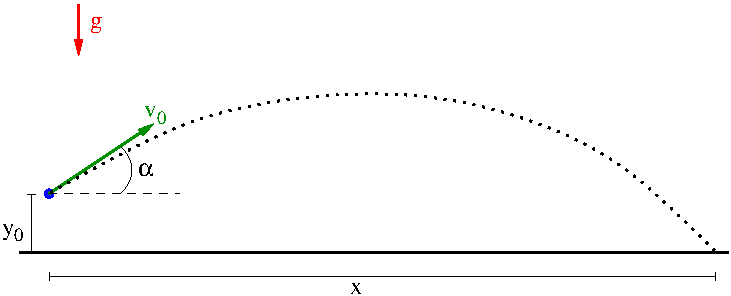
\includegraphics[scale=1]{rawfigs/projectile}
\vspace*{-8pt}
\caption{Object traveling with projectile motion. }
\label{fig:projectile}
\end{figure}


%Assume that we want to describe the motion of such an object, starting at time $t = 0$, ... and velocity that makes an angle $\alpha$ with the $x$-axis.


For this example, we assume that $h_0 =0$ m, $\alpha = \pi/4$ radians, $v_0 = 5$ m/s, all deterministic variables; and $g$ is the solution of the SIP described in Section \ref{sec:sip}.

Since a PDF is assigned to parameter $g$; thus, the output of the mathematical model (\ref{eq:fwd01}) becomes a random variable, thus we have a statistical forward problem. 

\subsection{The Input RV, QoI Function and Output RV}
 
The input random variable for the statistical forward problem is the acceleration of gravity $g$, which is also the solution (posterior PDF) of the inverse problem described in Section \ref{sec:sip}. The output random variable for this example is the distance $x$ traveled by an object in projectile motion. Note that, since there is uncertainty in the parameter $g$ ($g$ is given as a PDF), one can expect that this uncertainty will be propagated to $x$, which will also be given as a PDF.

Combining the expressions in Equation \ref{eq:fwd01} and rearranging them, we have that QoI function for $x$ %(i.e. the final model for the distance traveled by an object in projectile motion) 
is: 
\begin{equation}\label{eq:fp_deterministic}
x=\dfrac{ v_0 \cos \alpha }{g} \left( v_0  \sin \alpha  + \sqrt{ ( v_0  \sin \alpha)^2 + 2g\, y_0 }\right).                                                                                        
\end{equation}
where $y$ is the distance traveled and our quantity of interest (QoI). 


\subsection{Algorithms for solving the Statistical Forward Problem}




The Monte Carlo method is commonly used for analyzing uncertainty propagation, where the goal is to determine how random variation, lack of knowledge, or error affects the sensitivity, performance, or reliability of the system that is being modeled \cite{RoCa04}.

Monte Carlo works by using random numbers to sample, according to a PDF, the `solution space' of the problem to be solved.
Then, it iteratively evaluates a deterministic model using such sets of random numbers as inputs.


Monte Carlo is implemented in QUESO and it is the chosen algorithm to compute a sample of the output RV (the QoI) of the SFP for each given sample of the input RV. 

\section{Application Code}\label{sec:application_code}

The source code for the SIP and the SFP is composed of 7 files.
Three of them are common for both problems: \texttt{gravity\_main.C, gravity\_compute.h} and \texttt{gravity\_compute.C,}; they combine both problems and use the solution of the SIP (the posterior PDF for the gravity) as an input for the SFP and are presented, respectively, in Listings \ref{code:gravity_main}, \ref{code:gravity_compute_h} and \ref{code:gravity_compute_C}.
Two of files specifically  handle the SIP: \texttt{gravity\_likelihood.h}, and \texttt{gravity\_likelihood.C}, and are displayed in Listings \ref{code:gravity_like_h} and \ref{code:gravity_like_C}. Finally, the files specific for the SFP are \texttt{gravity\_qoi.h} and \texttt{gravity\_qoi.C}, and they are presented in Listings \ref{code:gravity_qoi_h} and \ref{code:gravity_qoi_C}.

\lstinputlisting[caption=File \texttt{gravity\_main.C.}, label=code:gravity_main, linerange={27-1000}]{../../trunk/examples/gravity/src/gravity_main.C}
 
\lstinputlisting[caption=File \texttt{gravity\_compute.h.}, label=code:gravity_compute_h, linerange={27-1000}]{../../trunk/examples/gravity/src/gravity_compute.h}

\lstinputlisting[caption={File \texttt{gravity\_compute.C}. The first part of the code (lines 37--113) handles the statistical forward problem, whereas the second part of the code (lines 115--163) handles the statistical forward problem.\\}, label=code:gravity_compute_C, linerange={27-1000},numbers=left]{../../trunk/examples/gravity/src/gravity_compute.C}

\lstinputlisting[caption=File \texttt{gravity\_likelihood.h}., label=code:gravity_like_h, linerange={27-1000}]{../../trunk/examples/gravity/src/gravity_likelihood.h}

\lstinputlisting[caption=File \texttt{gravity\_likelihood.C}., label=code:gravity_like_C, linerange={27-1000}]{../../trunk/examples/gravity/src/gravity_likelihood.C}

\lstinputlisting[caption=File \texttt{gravity\_qoi.h}., label=code:gravity_qoi_h, linerange={27-1000}]{../../trunk/examples/gravity/src/gravity_qoi.h}

\lstinputlisting[caption=File \texttt{gravity\_qoi.C}., label=code:gravity_qoi_C, linerange={27-96}]{../../trunk/examples/gravity/src/gravity_qoi.C}

\section{Application Input File}\label{sec:application_input_file}

QUESO reads an input file for solving statistical problems.
In the case of a SIP, it expects a list of options for MCMC, while in case of SFP it expects a list of options for Monte Carlo.

The most relevant options of an input file for the solution of a SIP using QUESO are displayed in Listing \ref{code:gravity_inp_sip}.
Note that the names of the variables have been designed to be informative:
\begin{description}\vspace{-8pt}
\item[ \texttt{env}:] refers to QUESO environment; \vspace{-8pt}
\item[ \texttt{ip}:] refers to inverse problem;\vspace{-8pt}
\item[ \texttt{mh}:] refers to Metropolis-Hastings;\vspace{-8pt}
\item[ \texttt{dr}:] refers to delayed rejection;\vspace{-8pt}
\item[ \texttt{am}:] refers to adaptive Metropolis;\vspace{-8pt}
\item[ \texttt{rawChain}:] refers to the raw, entire chain; \vspace{-8pt}
\item[ \texttt{filteredChain}:] refers to a filtered chain (related to a specified \texttt{lag});\vspace{-8pt}
\item[ \texttt{fp}:] refers to forward problem;\vspace{-8pt}
\item[ \texttt{mc}:] refers to Monte Carlo;\vspace{-8pt}
\item[ \texttt{pseq}:] refers to the parameter sequence; and\vspace{-8pt}
\item[ \texttt{qseq}:] refers to the quantity of interest sequence.
\end{description}

\lstinputlisting[caption=Some options for QUESO library used in application code (Listings \ref{code:gravity_main}-\ref{code:gravity_like_C})., label={code:gravity_inp_sip},]{../../trunk/examples/gravity/tests/test_2013_01_22/gravity_inv_fwd.inp}


 

Moreover, for the gravity inverse problem, one may notice that QUESO will use the Metropolis-Hastings algorithm to sample the posterior PDF
(indicated by the prefix \texttt{mh\_}in the variable names) without adaptive steps
(indicated by the zero value assigned to the variable \linebreak \texttt{ip\_mh\_am\_initialNonAdaptInterval}, which can also be achieved by setting zero to \linebreak
\verb+ip_mh_am_adaptInterval+) and with delayed rejection (indicated by the one-value assigned to the variable \texttt{ip\_mh\_dr\_maxNumExtraStages}).





 
\section{Application Compilation and Run}\label{sec:application_compilation}


Makefiles are special format files that together with the make utility will help one to compile and automatically build and manage projects (programs).
Listing \ref{code:makefile} presents a Makefile, named \texttt{Makefile\_example\_violeta}, that may be used to compile the code and create the executable \verb+gravity_gsl+. Naturally, it must be adapted to the user's settings, i.e., it has to have the correct paths for the user's libraries that were actually used to compile and install QUESO (see Sections \ref{sec:Pre_Queso}--\ref{sec:install_Queso_make}).

\lstinputlisting[caption={Makefile for the application code in Listings \ref{code:gravity_main}-\ref{code:gravity_like_C}},  label={code:makefile},language={bash}]{../../trunk/examples/gravity/src/Makefile_example_violeta}



Suppose the user either does not need to modify the Makefile presented in Listings \ref{code:makefile} or has already done so. Then, in order to compile, build and run the application code together  with its input file \verb+gravity_inv_fwd.inp+, presented in Listing~\ref{code:gravity_inp_sip}, the user simply needs to enter following commands, under QUESO build tree:
\begin{lstlisting}[caption={}, label={},language={bash}]
cd $HOME/queso_download/queso-0.46.0/examples/gravity/src
make -f Makefile_example_violeta
cd ../tests/test_2013_01_22
../../src/gravity_gsl gravity_inv_fwd.inp
\end{lstlisting}



% Then, in order to run the application code with \underline{no} modifications, together with its input file \verb+gravity_inv_fwd.inp+ presented in Listing~\ref{code:gravity_inp_sip}., one just needs to type the command line:
% \begin{lstlisting}[caption={}, label={},language={bash}]
% cd $HOME/LIBRARIES/QUESO-0.46.0/examples/gravity
% ./gravity_gsl gravity_inv_fwd.inp
% \end{lstlisting}
% 
% However, if any modification has been placed by the user, he/she must re-compile and build the code, before running it. For that, use suggest the use of a Makefile similar to the one presented in Listing \ref{code:makefile}, adapted to the user's current libraries. Such Makefile is located at QUESO build tree. Thus:
% \begin{lstlisting}[caption={}, label={},language={bash}]
% cd $HOME/queso_download/queso-0.46.0/examples/gravity/src
% make -f Makefile_example_violeta
% cd ../tests/test_2013_01_22
% ../../src/gravity_gsl gravity_inv_fwd.inp
% \end{lstlisting}

Alternatively, if the user is not interested in re-compiling and and building the code, he/she can simply run the executable created during QUESO installation, and, thus, located at QUESO installation tree: 
\begin{lstlisting}[caption={}, label={},language={bash}]
cd $HOME/LIBRARIES/QUESO-0.46.0/examples/gravity
./gravity_gsl gravity_inv_fwd.inp
\end{lstlisting}
 
In either case, the console output of the program is:
\begin{lstlisting}[caption={Console output of program \texttt{gravity\_gsl}}, label={code:console_output},language={bash}]
kemelli@violeta:~/LIBRARIES/QUESO-0.46.0/examples/gravity$ ./gravity_gsl gravity_inv_fwd.inp 
---------------------------------------------------------------------
QUESO Library: Version = 0.46.0 (4600)

Development Build

Build Date   = 2013-04-29 17:05
Build Host   = violeta
Build User   = kemelli
Build Arch   = x86_64-unknown-linux-gnu
Build Rev    = 38998M

C++ Config   = mpic++ -g -O2 -Wall

Trilinos DIR = 
GSL Libs     = -L/home/kemelli/LIBRARIES/gsl-1.15/lib -lgsl -lgslcblas -lm
GRVY DIR     = 
GLPK DIR     = 
HDF5 DIR     = /home/kemelli/LIBRARIES/hdf5-1.8.10
--------------------------------------------------------------------------------------------------------------
Beginning run at Mon Apr 29 17:27:32 2013

MPI node of worldRank 0 has fullRank 0, belongs to subEnvironment of id 0, and has subRank 0
MPI node of worldRank 0 belongs to sub communicator with full ranks 0
MPI node of worldRank 0 also belongs to inter0 communicator with full ranks 0, and has inter0Rank 0


Beginning run of 'Gravity + Projectile motion' example at Mon Apr 29 17:27:32 2013

 my fullRank = 0
 my subEnvironmentId = 0
 my subRank = 0
 my interRank = 0

Beginning 'SIP -> Gravity estimation' at Mon Apr 29 17:27:32 2013

Solving the SIP with Metropolis Hastings

Beginning 'SFP -> Projectile motion' at Mon Apr 29 17:27:33 2013

Solving the SFP with Monte Carlo

Ending run of 'Gravity + Projectile motion' example at Mon Apr 29 17:27:33 2013

Ending run at Mon Apr 29 17:27:33 2013
Total run time = 1 seconds
kemelli@violeta:~/LIBRARIES/QUESO-0.46.0/examples/gravity$ 
\end{lstlisting}


\subsection{Application Run with Several Processors}
\new{
Even though the application described in Section \ref{sec:application_code} is a serial code, it is possible to run it using more than one processor, i.e., in parallel mode. 
Supposing the user's workstation has $N_p=8$ processors, then, the user my choose to have $N_s =$ 8, 4 or 2 subenvironments. This complies with the requirement that the total number of processors in the environment must be a multiple of the specified number of subenvironments.

Thus, to build and run the application code with $N_p = 8$, and $N_s=8$ subenvironments, the must set the variable \texttt{env\_numSubEnvironments = 8} in the input file (Listing~\ref{code:gravity_inp_sip}) and enter the following command lines: 

}

\begin{lstlisting}[caption={}, label={},language={bash}]
cd $HOME/LIBRARIES/QUESO-0.46.0/examples/gravity/
mpirun -np 8 ./gravity_gsl gravity_inv_fwd.inp
\end{lstlisting}

\new{
The steps above will create a total number of 8 raw chains, of size defined by the variable \texttt{ip\_mh\_rawChain\_size}. QUESO internally combines these 8 chains into a single chain of size $8\; \times\,$\texttt{ip\_mh\_rawChain\_size} and saves it in a file named according to the variable \texttt{ip\_mh\_rawChain\_dataOutputFileName}. 
QUESO also provides the user with the option of writing each chain -- handled by its corresponding processor -- in a separate file, which is accomplished by setting the variable \texttt{ip\_mh\_rawChain\_dataOutputAllowedSet = 0 1 ... Ns-1}.\\

\noindent
{\bf Note:} Although the discussion in the previous paragraph refers to the raw chain of a SIP, the analogous is true for the filtered chains (SIP), and for the samples employed in the SFP (\texttt{ip\_mh\_filteredChain\_size},    \texttt{fp\_mc\_qseq\_size} and \texttt{fp\_mc\_qseq\_size}, respectively). 

}



\section{Application Results}\label{sec:application_results}

There are a few Matlab-ready commands that are very helpful tools for post-processing the data generated by QUESO when solving statistical inverse problems.
This section discusses the results computed by QUESO with the code of Section \ref{sec:application_code}, and shows how to use Matlab for the post-processing of such results. 

According to the specifications of the input file in Listing~\ref{code:gravity_inp_sip}, both a folder named \verb+outputData+ and a the following files should be generated:
\begin{verbatim}
display_env_sub0.txt  
sfp_gravity_p_seq.m   
sfp_gravity_p_seq_sub0.m  
sfp_gravity_qoi_seq.m 
sfp_gravity_qoi_seq_sub0.m  
sfp_gravity_sub0.m
sip_gravity_filtered_chain.m  
sip_gravity_filtered_chain_sub0.m 
sip_gravity_raw_chain.m    
sip_gravity_raw_chain_sub0.m
sip_gravity_sub0.m 
\end{verbatim}

%The names of the files have been chosen to be informative.


%In this case, only one sub-environment (processor) has been used, thus, only one file of the type \verb+display_env_sub*+ is generated.
%

In this section, a convenient capability of QUESO of internally handling possible conflicts in chain size is presented. Recalling the input file \verb+gravity_inv_fwd.inp+ presented in Listing~\ref{code:gravity_inp_sip}, one may notice that  the raw chain size for the SIP is chosen to have 20000 positions (\verb+ip_mh_rawChain_size = 20000+); the lag of the filtered chain is chosen to be 20 (\verb+ip_mh_filteredChain_lag = 20+) and the chain size for the SFP has 16384 positions (\verb+fp_mc_qseq_size = 16384+). Because the solution of the SIP, ie, the posterior PDF, is used as input PDF for the SFP, QUESO internally sets \verb+fp_mc_qseq_size = 20000+, as can be seen in the file \verb+display_env_sub0.txt+.  The file \verb+display_env_sub0.txt+ contains information from the subenvironment `0' that was generated during the run of the application code.

\subsection{Statistical Inverse Problem}


\subsubsection{Chain Plots}

It is quite simple to plot, using Matlab, the chain of positions used in the DRAM algorithm implemented within QUESO. 
The sequence of Matlab commands presented in Listing \ref{matlab:chain} generates the graphic depicted in Figure \ref{fig:sip_gravity_chain_pos_raw}.
Figure~\ref{fig:sip_gravity_chain_pos_filtered} is obtained analogously. % by loading \verb+sip_gravity_filtered_chain+ and using  \verb+ip_mh_filtChain_unified+ inside \verb+plot+.

\begin{lstlisting}[label=matlab:chain,caption={Matlab code for the chain plot.}]
% inside Matlab
>> sip_gravity_raw_chain
>> plot(ip_mh_rawChain_unified)
>> ylabel('\theta=g','fontsize',20);
>> xlabel('Number of positions','fontsize',20);
>> title('DRAM Chain Positions (raw)','fontsize',20);
\end{lstlisting}

\begin{figure}[htb]
\centering 
\subfigure[Raw chain]{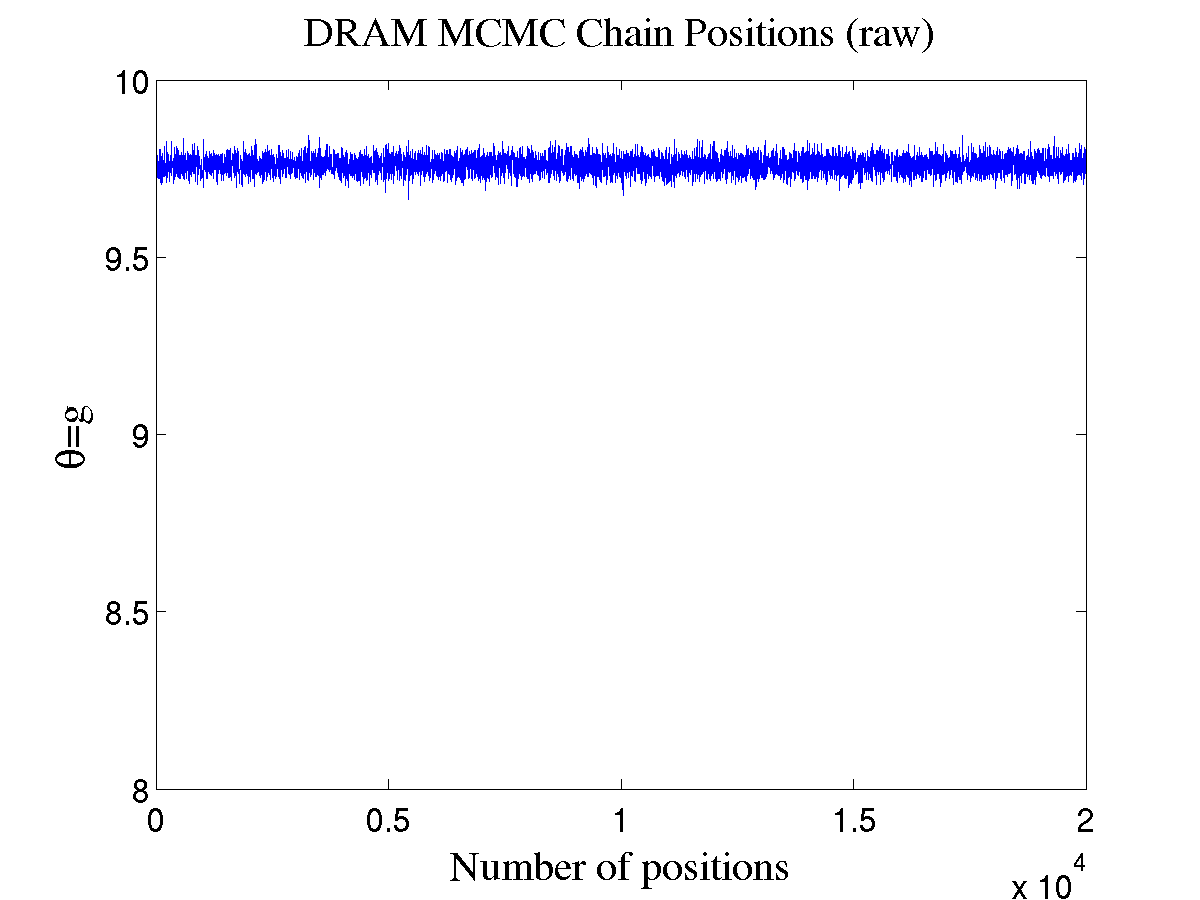
\includegraphics[scale=0.40]{rawfigs/sip_gravity_chain_pos_raw.png}\label{fig:sip_gravity_chain_pos_raw}}
\subfigure[Filtered chain]{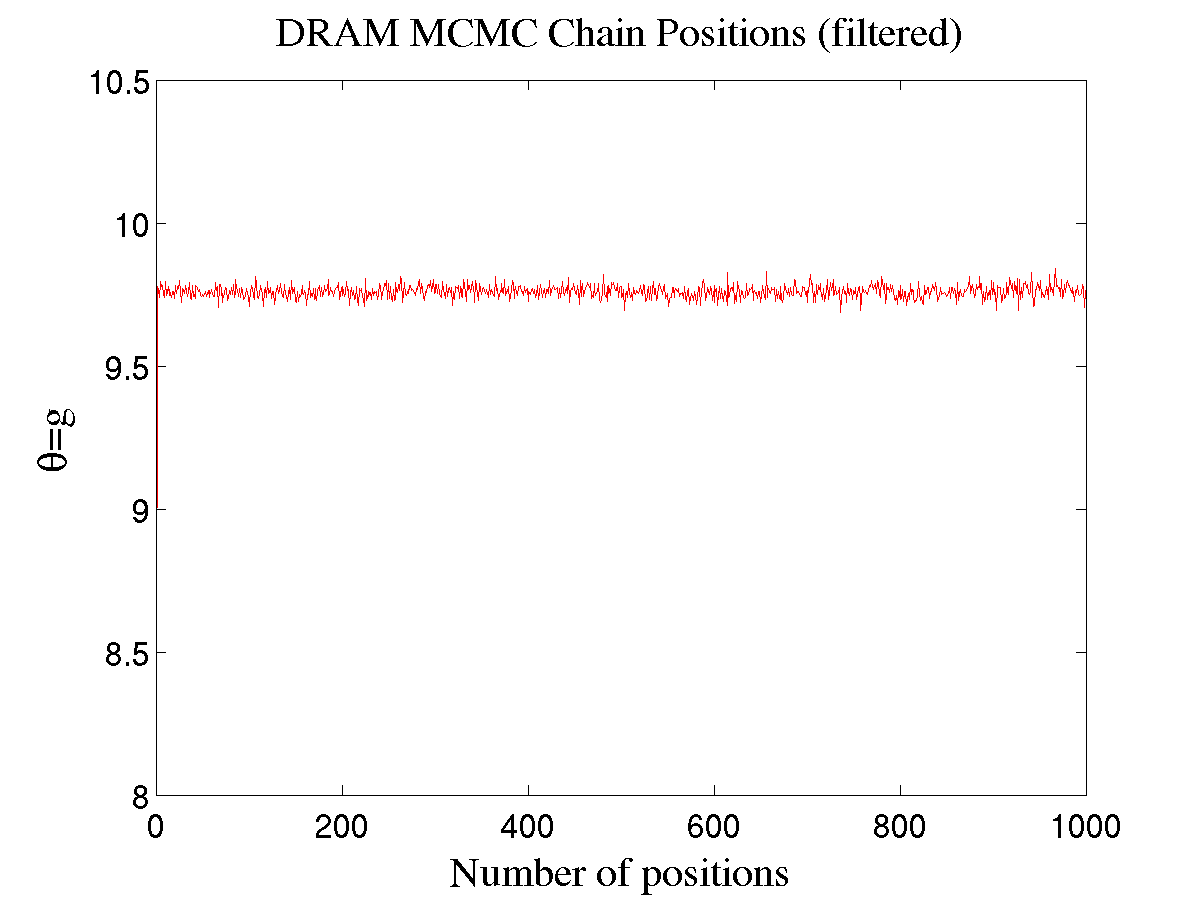
\includegraphics[scale=0.40]{rawfigs/sip_gravity_chain_pos_filt.png}\label{fig:sip_gravity_chain_pos_filtered}}
\vspace*{-10pt}
\caption{MCMC raw chain with \chainsizeresults{} positions and a filtered chain with lag of 20 positions.}
\end{figure}

\subsubsection{Histogram Plots}

In order to plot histograms of the parameter using either the raw chain or the filtered chain, you simply have to use the pre-defined Matlab function \verb+hist+.
%The Matlab code presented in Listing \ref{matlab:hist} below shows how to create the Figure \ref{fig:sip_gravity_hist_raw};
%once more, Figure \ref{fig:sip_gravity_hist_filtered} is obtained by making suitable adjustments on that code.
%
\begin{lstlisting}[label=matlab:hist,caption={Matlab code for the histogram plot.}]
% inside Matlab
>> sip_gravity_raw_chain
>> nbins=100;
>> hist(ip_mh_rawChain_unified,nbins)
>> title('Parameter Histogram (raw chain)','fontsize',20);
>> xlabel('Gravity (m/s^2)','fontsize',20);
>> ylabel('Frequency','fontsize',20);
>> grid on;
\end{lstlisting}

\begin{figure}[htb]
\centering 
\subfigure[Raw chain]{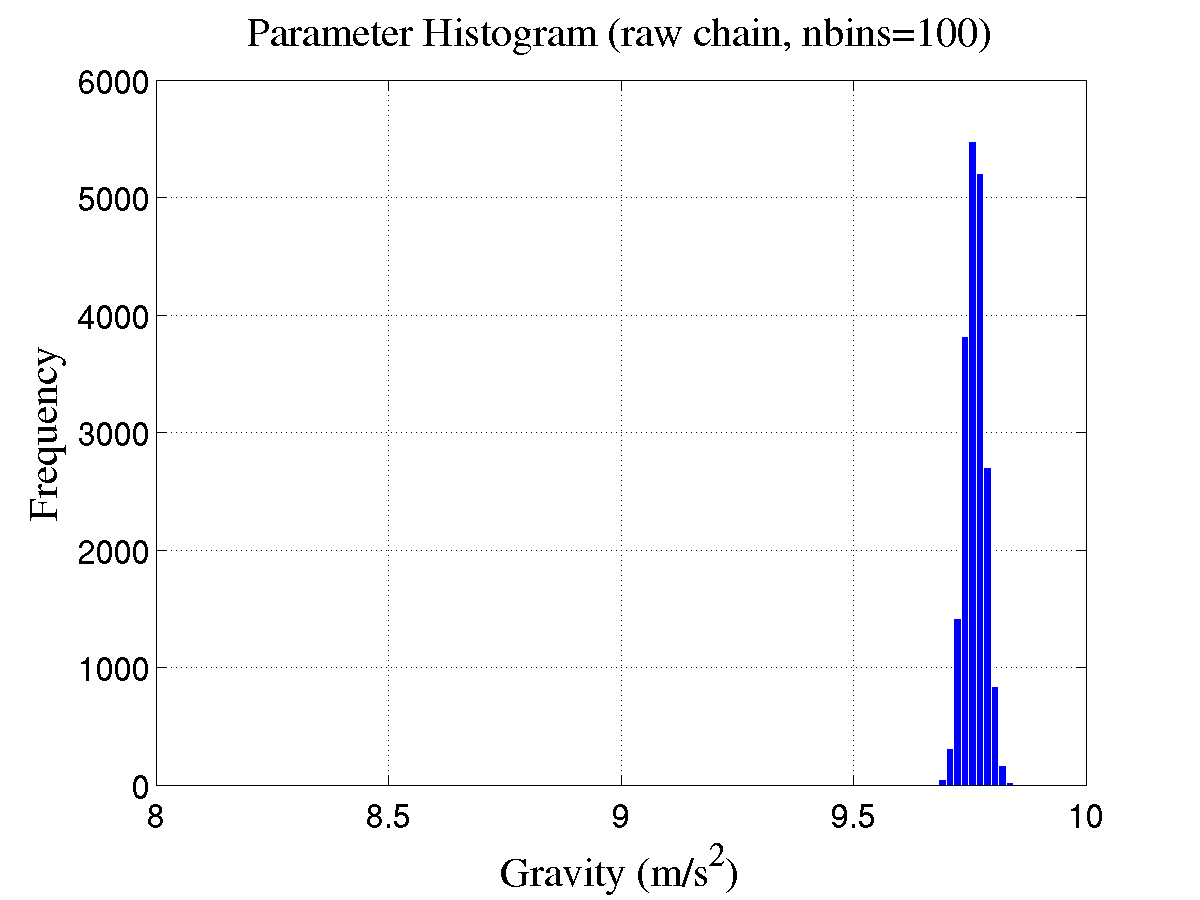
\includegraphics[scale=0.40]{rawfigs/sip_gravity_hist_raw.png}\label{fig:sip_gravity_hist_raw}}
\subfigure[Filtered chain]{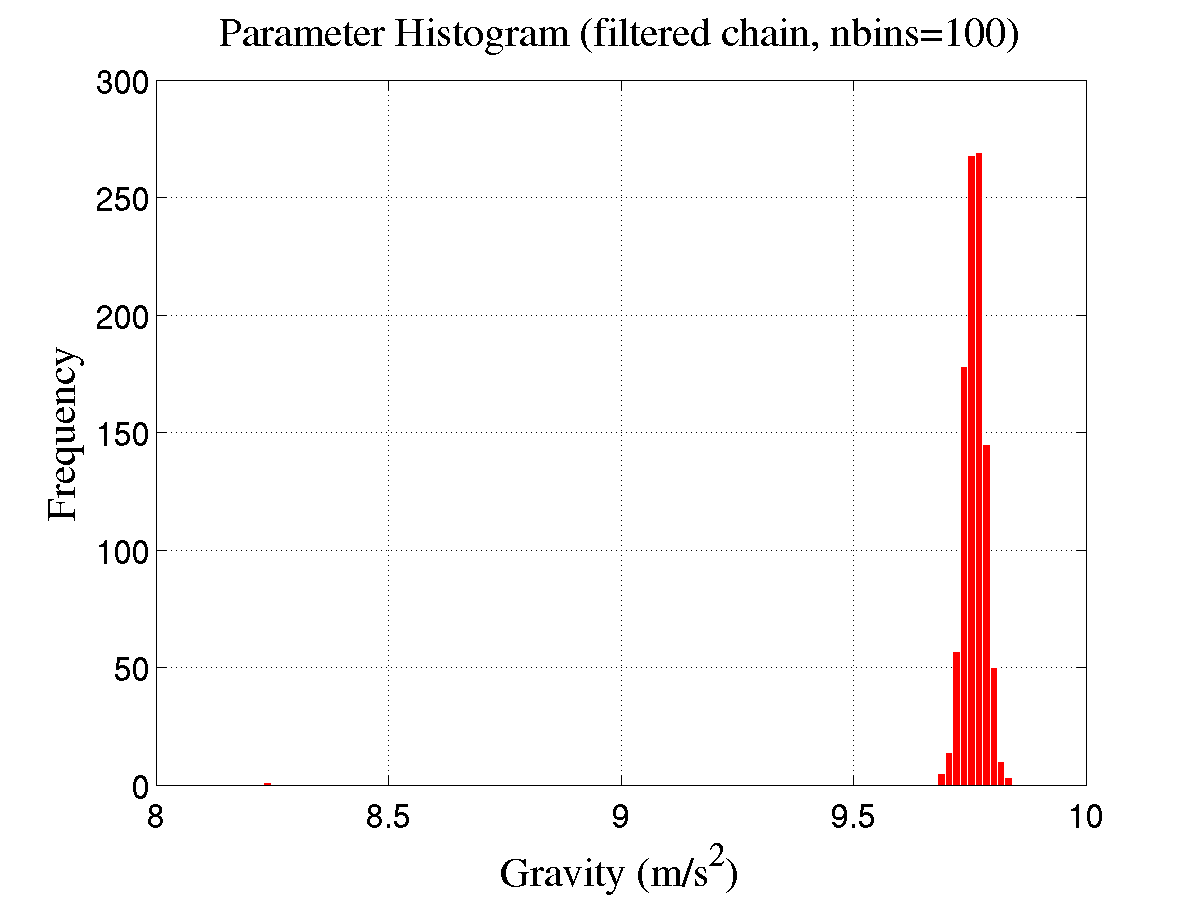
\includegraphics[scale=0.40]{rawfigs/sip_gravity_hist_filt.png}\label{fig:sip_gravity_hist_filtered}}
\vspace*{-10pt}
\caption{Histograms of parameter $\theta=g$. }
\end{figure}

\subsubsection{KDE Plots}

Matlab function \verb+ksdensity+ (Kernel smoothing density estimate) together with the option \verb+'pdf'+ may be used for plotting the KDE of the parameter.
\begin{lstlisting}[label=matlab:kde,caption={Matlab code for the KDE plot.}]
% inside Matlab
>> sip_gravity_raw_chain
>> [f,xi] = ksdensity(ip_mh_rawChain_unified,'function','pdf');
>> plot(xi,f,'-b','linewidth',3)
>> title('Parameter Kernel Density Estimation','fontsize',20);
>> xlabel('Gravity (m/s^2)','fontsize',20);
>> ylabel('KDE','fontsize',20);
>> grid on;
\end{lstlisting}

%Figure \ref{fig:sip_gravity_kde_raw} is created by using Matlab commands presented in Listing \ref{matlab:kde} above.
\begin{figure}[htpb]
\centering 
\subfigure[Raw chain]{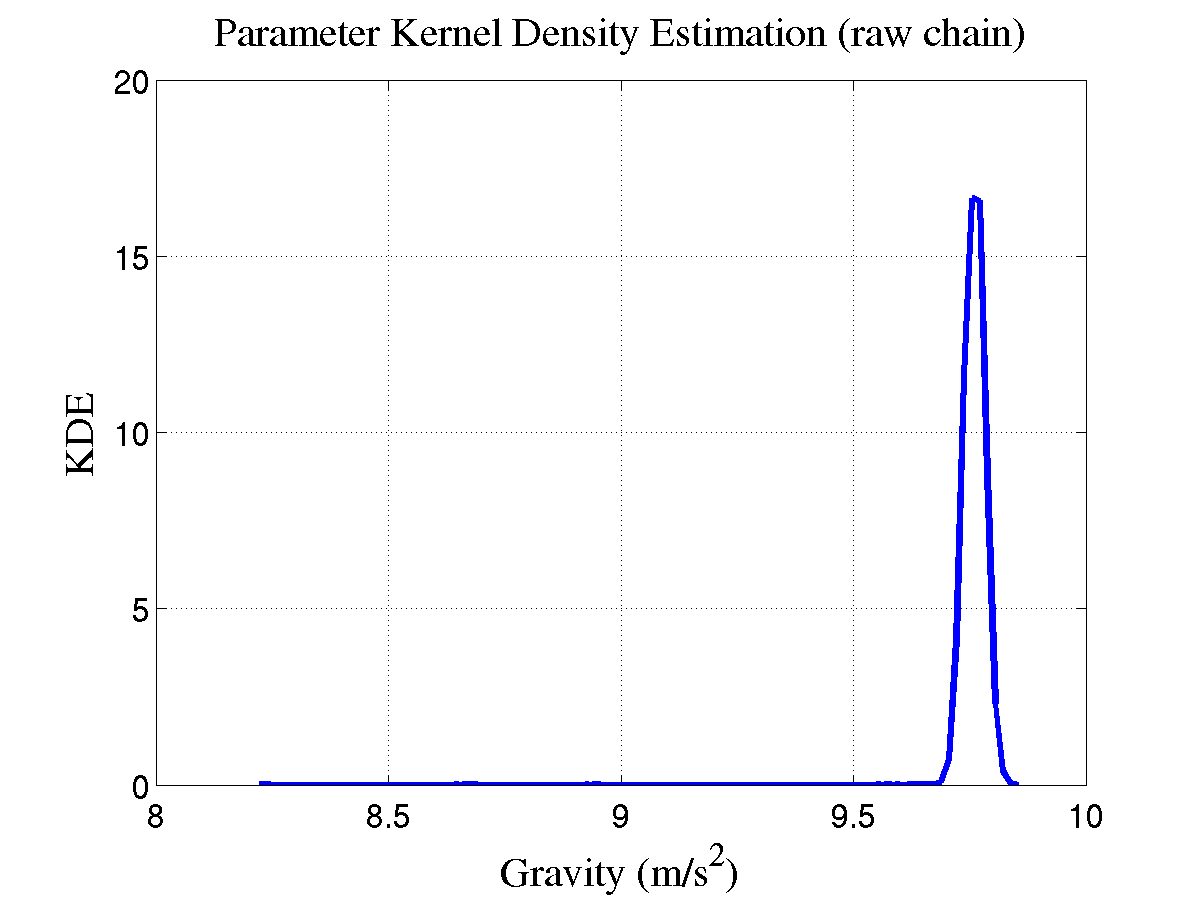
\includegraphics[scale=0.40]{rawfigs/sip_gravity_kde_raw.png}\label{fig:sip_gravity_kde_raw}}
\subfigure[Filtered chain]{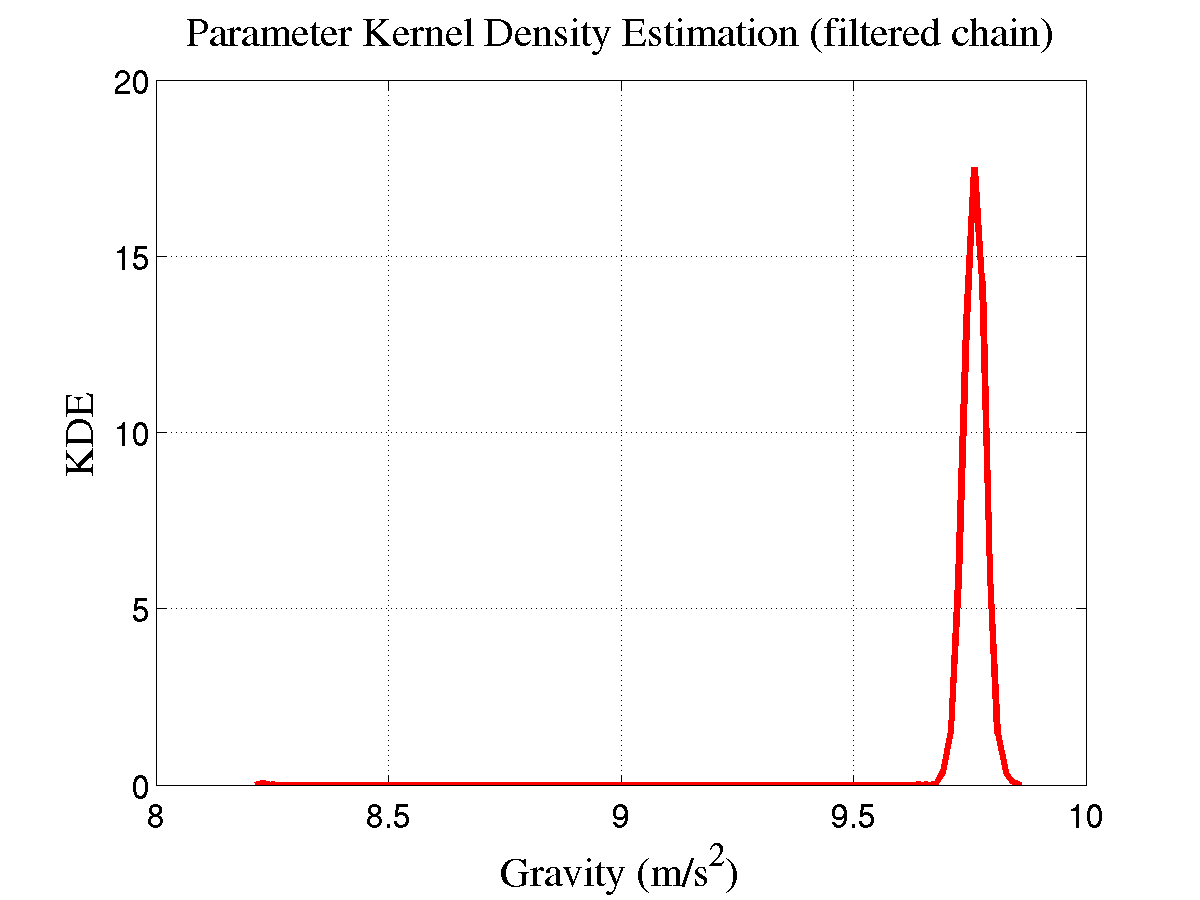
\includegraphics[scale=0.40]{rawfigs/sip_gravity_kde_filt.png}\label{fig:sip_gravity_kde_filtered}}
\vspace*{-10pt}
\caption{Kernel Density Estimation. }
\end{figure}


% \subsubsection{Checking a KDE Plot Against Brute-Force Plot of the Likelihood Function}
% 
% See Figure \ref{fig:sip_gravity_compare_brute_force_unnormal}.
% %Figures \ref{fig:sip_gravity_compare_brute_force_unnormal} and \ref{fig:sip_gravity_compare_brute_force_normal} depict unnormalized and normalized KDE distributions
% %comparing the solution of the SIP provided by QUESO ($\pi_{\text{post}} (g)$) and the analytical (brute force) distribution.
% 
% \begin{figure}[htpb]
% \centering 
% %\subfigure[Unnormalized]{\includegraphics[scale=0.40]{figs/gravity_likelihood_brute_force_compare_post_pdf_0.png}\label{fig:sip_gravity_compare_brute_force_unnormal}}
% %\subfigure[Normalized]{\includegraphics[scale=0.40]{figs/gravity_likelihood_brute_force_compare_post_pdf_normalized0.png}\label{fig:sip_gravity_compare_brute_force_normal}}
% \subfigure{\includegraphics[scale=0.40]{figs/gravity_likelihood_brute_force_compare_post_pdf_0.png}\label{fig:sip_gravity_compare_brute_force_unnormal}}
% \vspace*{-10pt}
% \caption{Comparison of the posterior KDE for $g$ against the brute force calculation of the likelihood on a regular grid on $g$.
% }
% \end{figure}
% 
% %The code had to be slightly modified in order to replace QUESO sampling from the uniform distribution for the gravity with what we call a `brute force sampling'.
% %This brute force `sampling'  consists of recovering a pre-defined amount of values for $g$ from an equally spaced interval.
% %This is accomplished in lines 75 -- 100 of code \ref{code:gravity_compute_bruteforce_C}: it replaces Steps 4-6 (lines 100-150)
% %of the original application code provided in Algorithm \ref{code:gravity_compute_C}.
% 
% %\lstinputlisting[caption={Application code modified to `brute force' sampling from pre-defined interval.}, label={code:gravity_compute_bruteforce_C},  linerange={28-1000}]{../../brute_force/gravity_compute.C}
%  
% %Once more, Matlab function \verb+ksdensity+ (Kernel smoothing density estimate) may be used for plotting the KDE of the parameter.
% %The Matlab code below is responsible for the generation of Figure \ref{fig:sip_gravity_compare_brute_force_unnormal}.
% %Note that it reads the file \verb+gravity_likeli_brute_force.dat+, which is an output of the brute force code depicted in Listing \ref{code:gravity_compute_bruteforce_C}.
% %%
% %\begin{lstlisting}[label=matlab:kde_bruteforce,caption={Matlab code for the comparison of KDE plot from QUESO and `brute force'.}]
% %% inside Matlab
% %>> [g,like]=textread('gravity_likeli_brute_force.dat', '%f %f' );
% %>> [f,xi] = ksdensity(ip_mh_rawChain_unified,'function','pdf');
% %>> [haxes,hline1,hline2] = plotyy(xi,f,g,exp(like),'plot', 'plot');
% %>> axes(haxes(1));
% %>> ylabel('\pi_{post}(g) - QUESO/raw chain','fontname', 'Times', 'fontsize',20);
% %>> axes(haxes(2));
% %>> ylabel('\pi_{like}(g) -  brute force','fontname', 'Times', 'fontsize',20);
% %>> grid on;
% %>> title('Unnormalized distributions','fontname', 'Times', 'fontsize',20);
% %>> set(hline1,'linewidth',3);
% %>> set(hline2,'linewidth',3);
% %\end{lstlisting}


\subsubsection{CDF Plots}

Matlab function \verb+ksdensity+ (Kernel smoothing density estimate) with \verb+'cdf'+ option may also be used for plotting the Cumulative Distribution Function of the parameter.


\begin{lstlisting}[label=matlab:cdf,caption={Matlab code for the CDF plot.}]
% inside Matlab
>> sip_gravity_raw_chain
>> [f,xi] = ksdensity(ip_mh_rawChain_unified,'function','cdf');
>> plot(xi,f,'-b','linewidth',3)
>> title('Parameter Cumulative Distribution Function','fontsize',20);
>> xlabel('Gravity (m/s^2)','fontsize',20);
>> ylabel('CDF','fontsize',20);
>> grid on;
\end{lstlisting}

%Similarly, Figure \ref{fig:sip_gravity_cdf_raw} is created by using above Matlab commands.
\begin{figure}[ht]
\centering 
\subfigure[Raw chain]{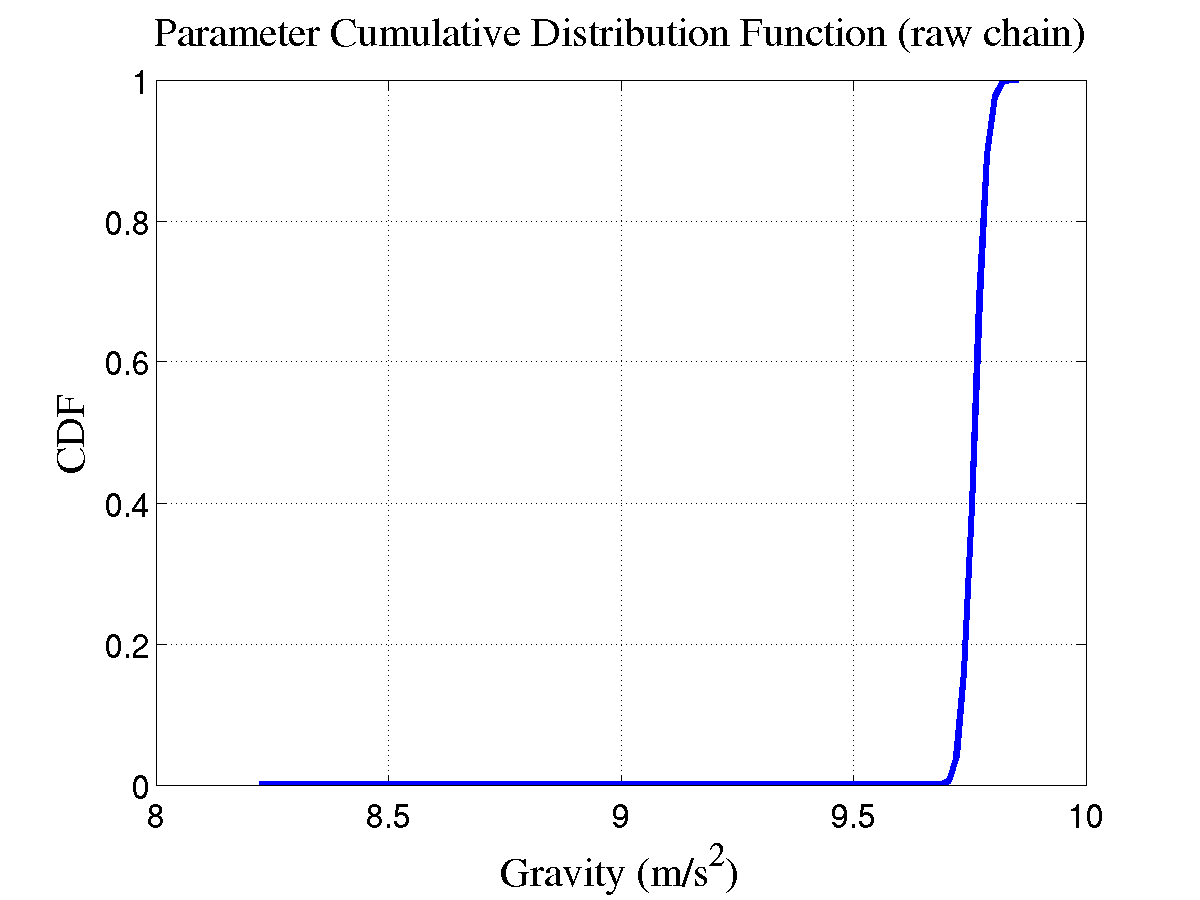
\includegraphics[scale=0.40]{rawfigs/sip_gravity_cdf_raw.png}\label{fig:sip_gravity_cdf_raw}}
\subfigure[Filtered chain]{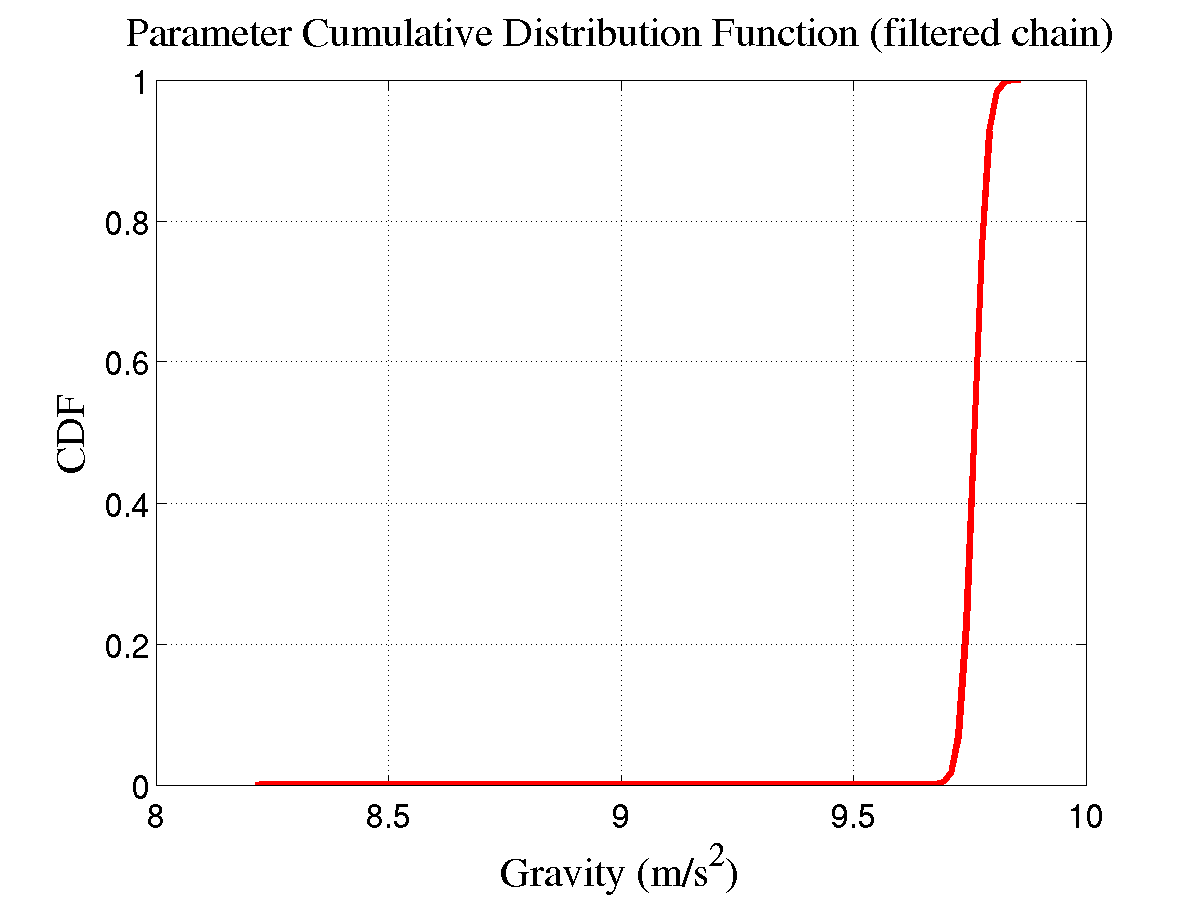
\includegraphics[scale=0.40]{rawfigs/sip_gravity_cdf_filt.png}\label{fig:sip_gravity_cdf_filtered}}
\vspace*{-10pt}
\caption{Cumulative Distribution Function. }
\end{figure}

\subsubsection{Autocorrelation Plots}

The code presented in Listing \ref{matlab:autocorr} uses matlab function \verb+autocorr+ to generate Figure \ref{fig:sip_gravity_autocorrelation_raw_filt}
which presents the autocorrelation of the parameter $g$ in both cases: raw and filtered chain.

\begin{lstlisting}[label=matlab:autocorr,caption={Matlab code for the autocorrelation plots.}]
% inside Matlab
>> sip_gravity_raw_chain
>> sip_gravity_filtered_chain
>> nlags=10;
>> [ACF_raw,lags,bounds]= autocorr(ip_mh_rawChain_unified, nlags, 0);
>> [ACF_filt,lags,bounds]=autocorr(ip_mh_filtChain_unified,nlags, 0);
>> plot(lags,ACF_raw,'bo-',lags,ACF_filt,'r*-','linewidth',3);
>> ylabel('Autocorrelation for \theta=g','fontsize',20);
>> xlabel('Lag','fontsize',20);
>> title('Parameter Autocorrelation','fontsize',20);
>> grid on;
>> h=legend('raw chain','filtered chain','location','northeast');
>> set(h,'fontsize',16);
\end{lstlisting}

\begin{figure}[htpb]
\centering
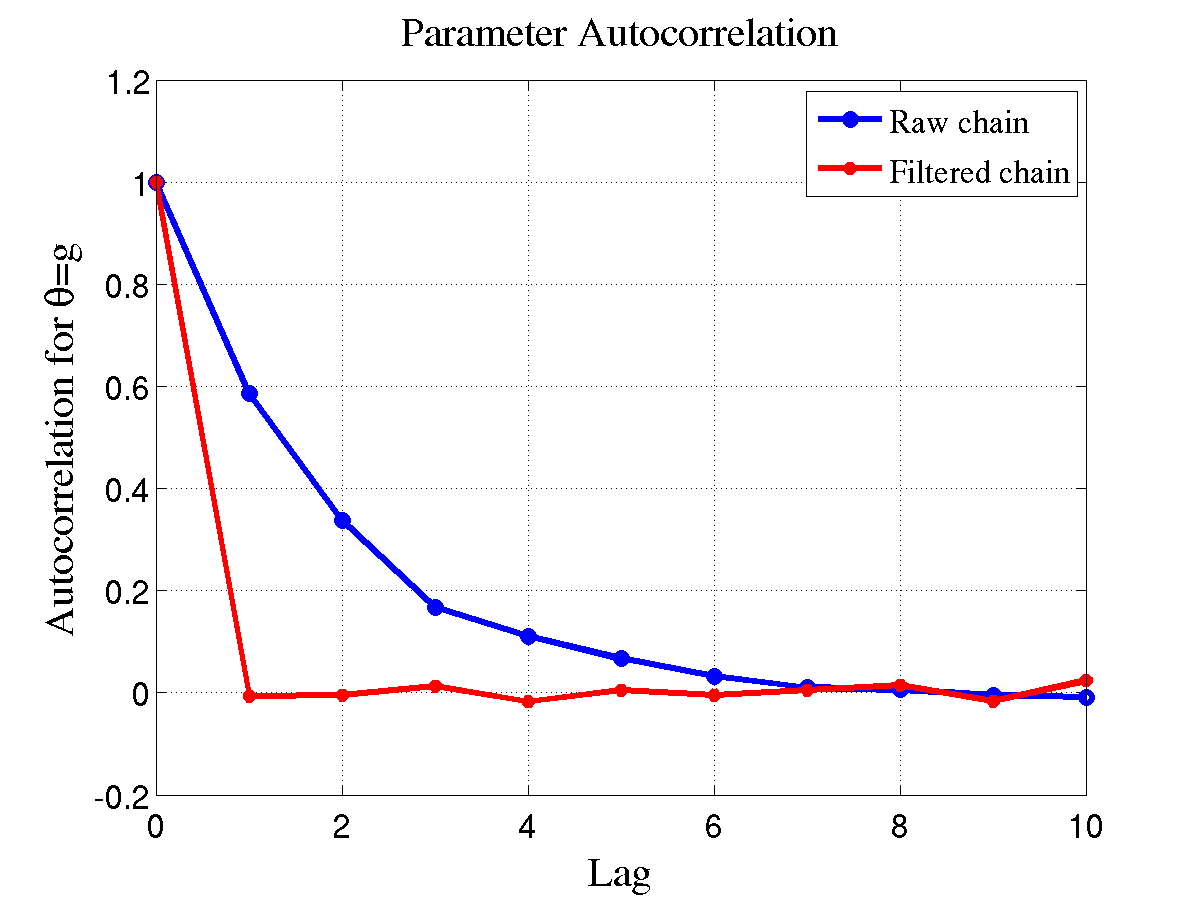
\includegraphics[scale=0.40]{rawfigs/sip_gravity_autocorrelation_raw_filt.png}
\vspace{-8pt}
\caption{
Autocorrelation plots. }
\label{fig:sip_gravity_autocorrelation_raw_filt}
\end{figure}

\subsubsection{Covariance and Correlation Matrices}

Matlab function \verb+cov+ calculates the covariance matrix for a data matrix (where each column represents a separate quantity), and \verb+corr+ calculates the correlation matrix.
Since our statistical inverse problem has only one parameter (the acceleration $g$ due to gravity), both covariance and correlation matrices have dimension $1 \times 1$, i.e., they are scalars.

\begin{lstlisting}[label=matlab:cov_matrix,caption={Matlab code for finding the covariance matrix.}]
% inside Matlab
>> sip_gravity_raw_chain;
>> cov_matrix_g = cov(ip_mh_rawChain_unified)
   
cov_matrix_g =

   6.8709e-04
>> corr_matrix_g = corr(ip_mh_rawChain_unified)

corr_matrix_g =

     1
>>
\end{lstlisting}


\subsection{Statistical Forward Problem}


\subsubsection{Chain Plots}

It is quite simple to plot, using Matlab, the chain of positions generated by the Monte Carlo algorithm implemented within QUESO and called during the solution of the statistical forward problem. 
%The sequence of Matlab commands presented in Listing \ref{matlab:chain_qoi} generates the graphic depicted in Figure~\ref{fig:sfp_gravity_chain}. 

\begin{lstlisting}[label=matlab:chain_qoi,caption={Matlab code for the chain plot.}]
% inside Matlab
>> sfp_gravity_qoi_seq.m
>> plot(fp_mc_QoiSeq_unified);
>> ylabel('QoI','fontsize',20);
>> xlabel('Number of positions','fontsize',20);
>> title('MC Chain Positions','fontsize',20);
\end{lstlisting}

\begin{figure}[htb]
\centering 
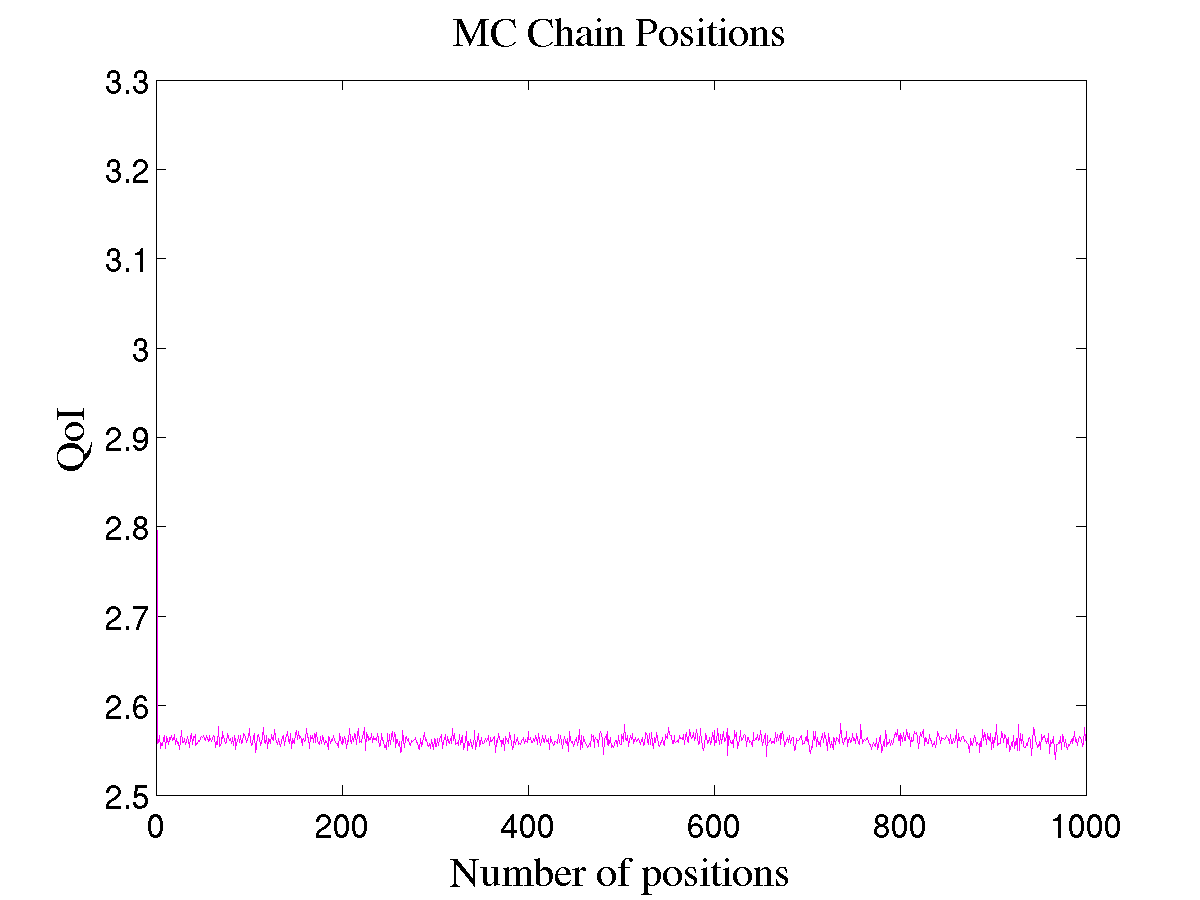
\includegraphics[scale=0.40]{rawfigs/sfp_gravity_chain_pos.png}
\vspace*{-10pt}
\caption{MC chain positions for the QoI.}
\label{fig:sfp_gravity_chain}
\end{figure}

\subsubsection{Histogram Plots}

In order to plot a histogram of the QoI, you may use the pre-defined Matlab function \verb+hist+.
%The Matlab code presented in Listing \ref{matlab:hist_qoi} below shows how to create the Figure~\ref{fig:sfp_gravity_hist}.
%
\begin{lstlisting}[label=matlab:hist_qoi,caption={Matlab code for the QoI histogram plot.}]
>> sfp_gravity_qoi_seq.m
>> nbins=100;
>> hist(fp_mc_QoiSeq_unified);
>> title('QoI Histogram','fontsize',20);
>> xlabel('Distance traveled (m)','fontsize',20);
>> ylabel('Frequency','fontsize',20);
>> grid on;
\end{lstlisting}

\begin{figure}[htb]
\centering 
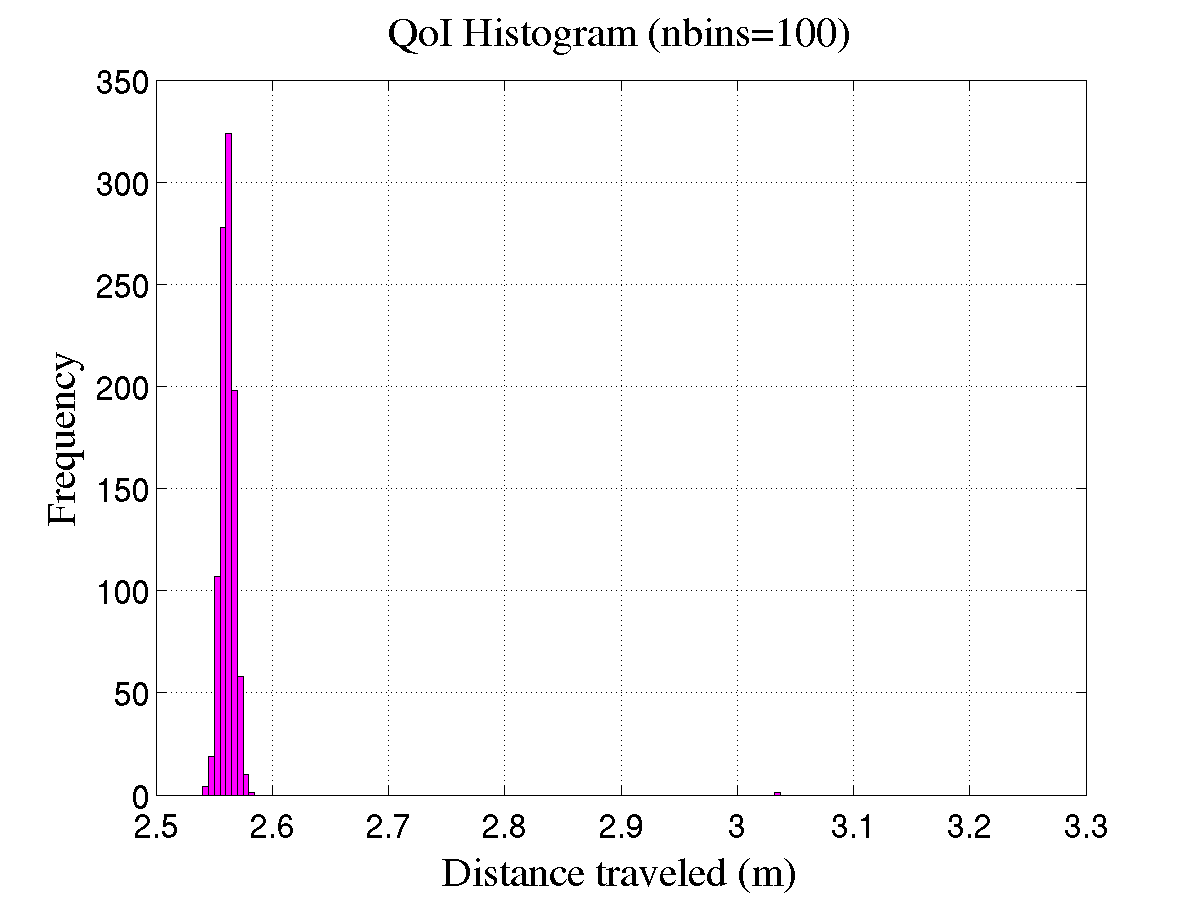
\includegraphics[scale=0.40]{rawfigs/sfp_gravity_hist.png}
\vspace{-10pt}
\caption{Histogram of QoI $=d$.}
\label{fig:sfp_gravity_hist}
\end{figure}

\subsubsection{KDE Plots}

Matlab function \verb+ksdensity+ (Kernel smoothing density estimate) together with the option \verb+'pdf'+ may be used for plotting the KDE of the he QoI.
\begin{lstlisting}[label=matlab:kde_qoi,caption={Matlab code for the QoI KDE plot.}]
% inside Matlab
>> sfp_gravity_qoi_seq.m
>> [f,xi] = ksdensity(fp_mc_QoiSeq_unified,'function','pdf');
>> plot(xi,f,'-b','linewidth',3)
>> title('QoI Kernel Density Estimation ','fontsize',20);
>> xlabel('Distance traveled (m)','fontsize',20);
>> ylabel('KDE','fontsize',20);
>> grid on;
\end{lstlisting}

\begin{figure}[htpb]
\centering 
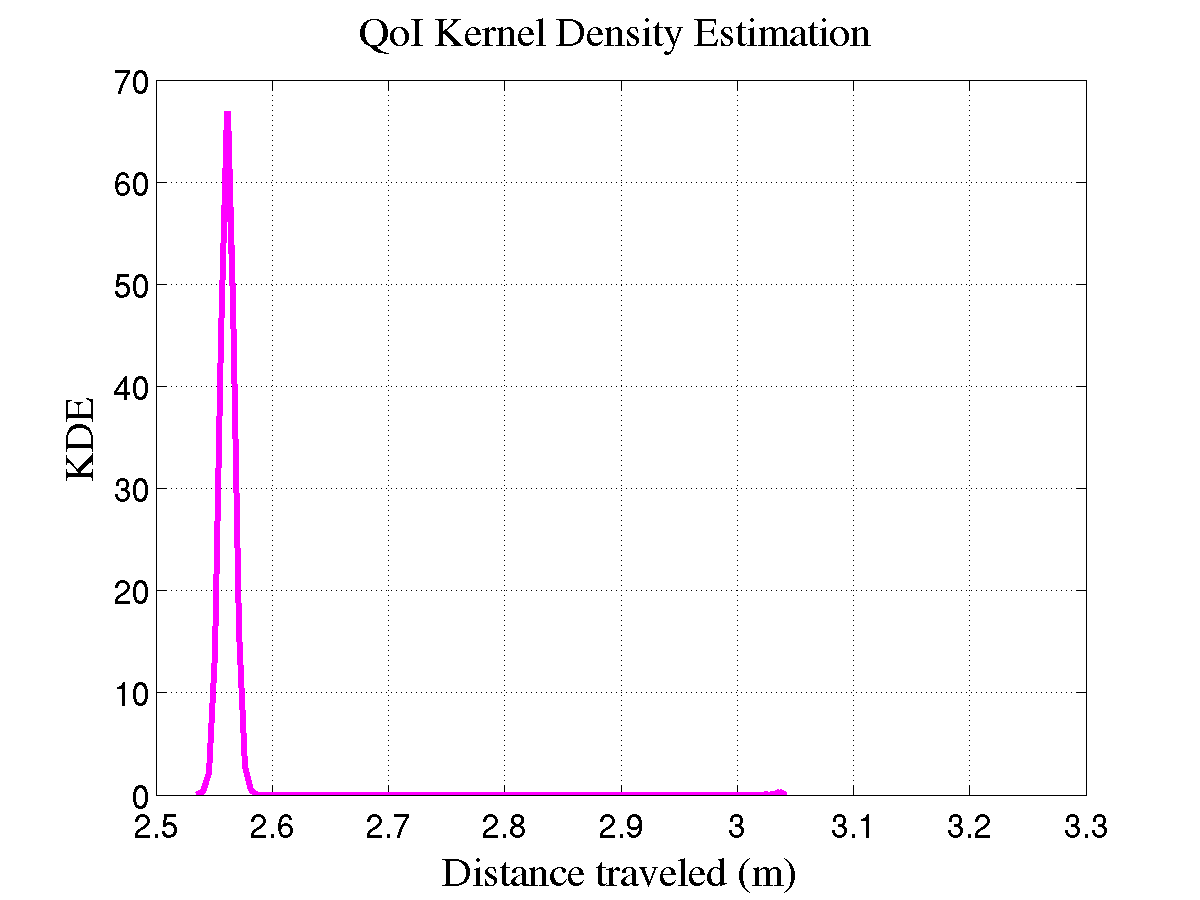
\includegraphics[scale=0.40]{rawfigs/sfp_gravity_kde.png}
\vspace*{-10pt}
\caption{Kernel Density Estimation.}
\label{fig:sfp_gravity_kde}
\end{figure}

\subsubsection{CDF Plots}

Matlab function \verb+ksdensity+ (Kernel smoothing density estimate) with \verb+'cdf'+ option may also be used for plotting the Cumulative Distribution Function of the QoI.

\begin{lstlisting}[label=matlab:cdf_qoi,caption={Matlab code for the QoI CDF plot.}]
% inside Matlab
>> sfp_gravity_qoi_seq.m
>> [f,xi] = ksdensity(fp_mc_QoiSeq_unified,'function','cdf');
>> plot(xi,f,'-b','linewidth',3)
>> title('QoI Cumulative Distribution Function ','fontsize',20);
>> xlabel('Distance traveled (m)','fontsize',20);
>> ylabel('CDF','fontsize',20);
>> grid on;
\end{lstlisting}

\begin{figure}[htpb]
\centering 
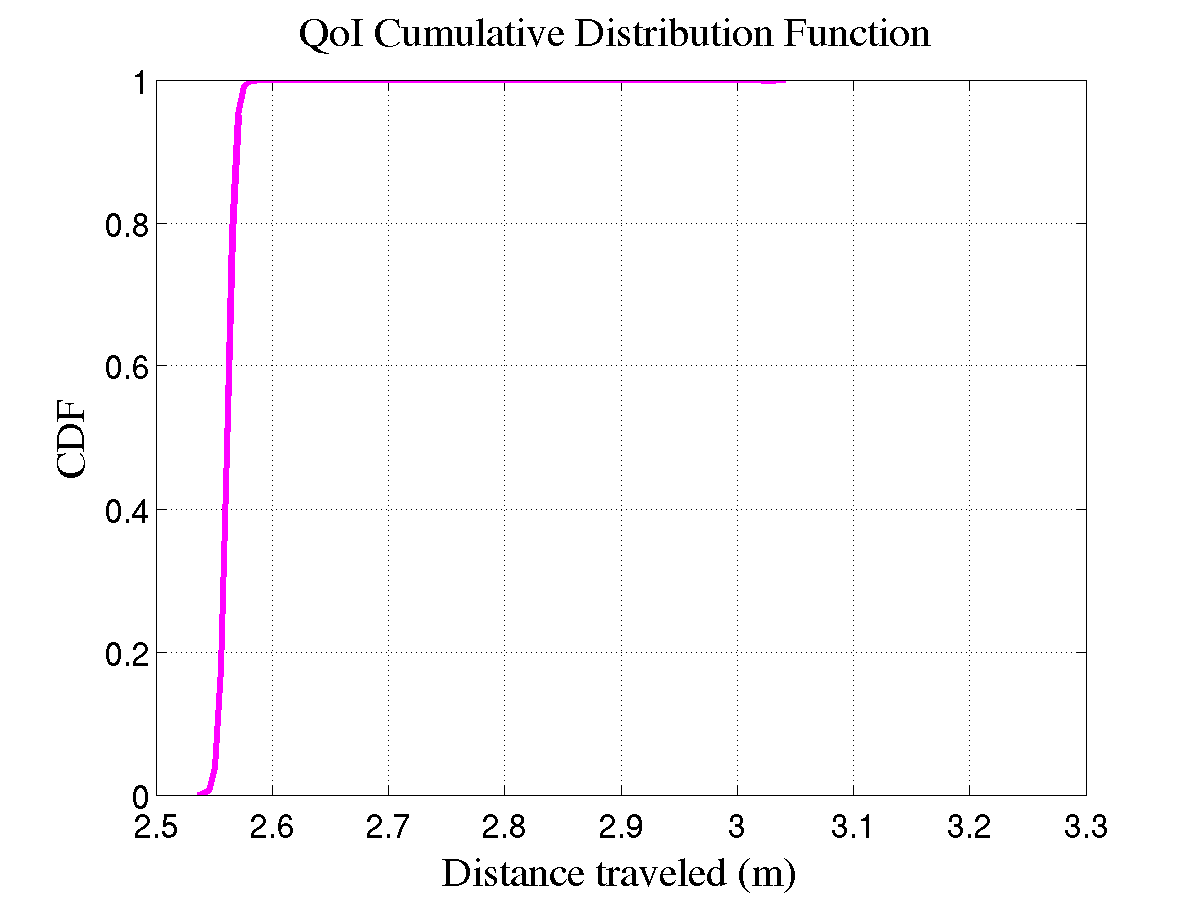
\includegraphics[scale=0.40]{rawfigs/sfp_gravity_cdf.png}
\vspace*{-10pt}
\caption{Cumulative Distribution Function.}
\label{fig:sfp_gravity_cdf}
\end{figure}

\subsubsection{Autocorrelation Plots}

The code presented in Listing \ref{matlab:autocorr_qoi} uses Matlab function \verb+autocorr+ to generate Figure \ref{fig:sfp_gravity_autocorrelation},
which presents the autocorrelation of the QoI $d$.

\begin{lstlisting}[label=matlab:autocorr_qoi,caption={Matlab code for the QoI autocorrelation plot.}]
% inside Matlab
>> sfp_gravity_qoi_seq.m
>> nlags=10;
>> [ACF, lags, bounds] = autocorr(fp_mc_QoiSeq_unified, nlags, 0);
>> plot(lags,ACF,'bo-','linewidth',3);
>> ylabel('Autocorrelation for QoI = d','fontsize',20);
>> xlabel('Lag','fontsize',20);
>> title('QoI Autocorrelation','fontsize',20);
>> grid on;
\end{lstlisting}

\begin{figure}[htb]
\centering
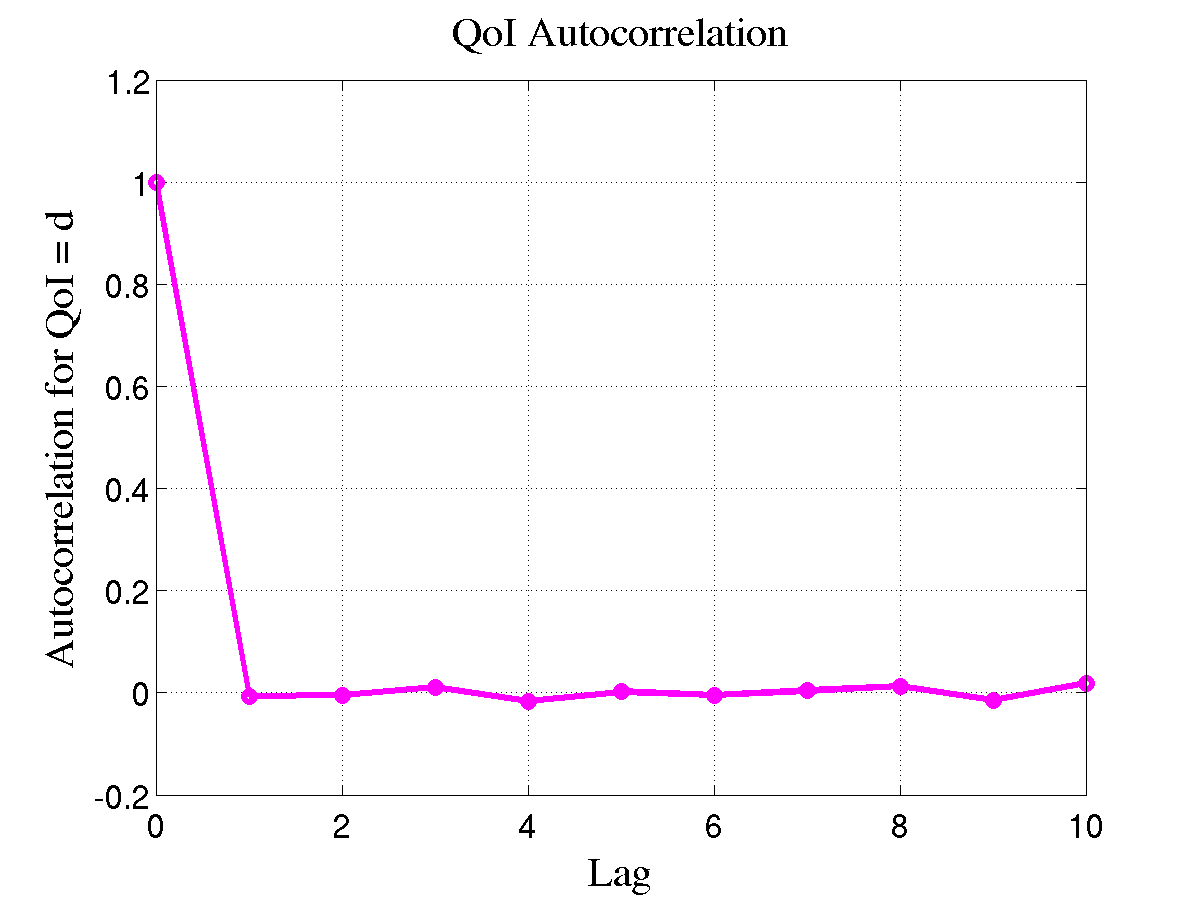
\includegraphics[scale=0.40]{rawfigs/sfp_gravity_autocorrelation.png}
\vspace*{-10pt}
\caption{Autocorrelation plot.}
\label{fig:sfp_gravity_autocorrelation}
\end{figure}

\subsubsection{Covariance and Correlation Matrices}

For a matrix input \verb+X+, where each row is an observation, and each column is a variable, the Matlab function \verb+cov(X)+ may be used to calculate the covariance matrix.
%The command \verb+diag(cov(X))+ is a vector of variances for each column, and, therefore, \verb+sqrt(diag(cov(X)))+ is a vector of standard deviations.  

Thus,  in order to calculated the covariance matrix between the parameter and the quantity of interest sequences generated by Monte Carlo sampler with QUESO,
one may simply define \verb+X=[fp_mc_ParamSeq_unified fp_mc_QoiSeq_unified]+.
The code presented in Listing \ref{matlab:cov_pqoi} shows the usage of Matlab commands for finding such the matrix.

\begin{lstlisting}[label=matlab:cov_pqoi,caption={Matlab code for the matrix of covariance between parameter $g$ and QoI $d$.}]
% inside Matlab
>> sfp_gravity_qoi_seq;
>> sfp_gravity_p_seq;
>> X=[fp_mc_ParamSeq_unified fp_mc_QoiSeq_unified];
>> cov_p_QoI = cov(X)

cov_p_QoI =
	  [ 2.826e-03 	-8.555e-04 ] 
	  [-8.555e-04 	 2.599e-04 ]

\end{lstlisting}

Analogously, the Matlab function \verb+corrcoef(X)+ returns a matrix of correlation coefficients calculated from an input matrix \verb+X+ whose rows are observations and whose columns are variables.
In order to calculated the correlation matrix between the parameter and the QoI sequences, one may simply define \verb+X=[fp_mc_ParamSeq_unified fp_mc_QoiSeq_unified]+.
% The matrix R = corrcoef(X) is related to the covariance matrix C = cov(X) b

\begin{lstlisting}[label=matlab:corr_param_qoi,caption={Matlab code for the matrix of correlation between parameter $g$ and quantity of interest $d$.}]
% inside Matlab
>> sfp_gravity_qoi_seq;
>> sfp_gravity_p_seq;
>> X=[fp_mc_ParamSeq_unified fp_mc_QoiSeq_unified];
>> corr_p_QoI = corrcoef(X)

corr_p_QoI =
	  [ 1.000e+00 	-9.981e-01 ] 
	  [-9.981e-01 	 1.000e+00 ]
>>
\end{lstlisting}


